\documentclass[12pt,a4paper]{article}

% Encoding og spraak
\usepackage[utf8]{inputenc}
\usepackage[T1]{fontenc}
\usepackage[nynorsk]{babel}

% Typografi
\usepackage{mathpazo}
\usepackage{microtype}

% Layout
\usepackage{geometry}
\geometry{a4paper, margin=2.5cm}
\usepackage{setspace}
\onehalfspacing

% Figurar og tabellar
\usepackage{graphicx}
\usepackage{float}
\usepackage{caption}
\usepackage{subcaption}
\usepackage{booktabs}
\usepackage{tabularx}

% Referansar (APA 7)
\usepackage[natbibapa]{apacite}
\usepackage{hyperref}
\hypersetup{
    colorlinks=true,
    linkcolor=black,
    citecolor=black,
    urlcolor=blue
}

% Diverse
\usepackage{csquotes}
\usepackage{amsmath}
\usepackage{enumitem}

% -------------------------------------------------------------------
\title{Form Follows Fitness:\\
\large Empirisk grunnlag for eit evolusjon\ae{}rt rammeverk i estetiske fag\\[0.5em]
\normalsize Del IV i ein PhD-serie om form, materialitet og industridesign}

\author{Iver Raknes Finne\\
\small Institutt for design, Arkitektur- og designh\o{}gskolen i Oslo (AHO)\\
\small\texttt{iver.finne@aho.no}}

\date{Mars 2026}

\begin{document}
\maketitle

% -------------------------------------------------------------------
\begin{abstract}
\noindent
Det modernistiske dogmet \enquote{form follows function} impliserer at form er deduserbar fr\aa{} funksjon. Denne artikkelen falsifiserer dette empirisk ved \aa{} analysere 93 stolar fr\aa{} Nasjonalmuseet si samling (1632--2018) gjennom 21~geometriske og 30~materielle eigenskapar utrekna fr\aa{} 3D-modellar. Analysen viser at funksjon er \emph{konstant}, alle objekta er stolar, medan form varierer radikalt: symmetri spenner 15~gonger, djupn 3~gonger, og kompaktheit 2.6~gonger. Informasjonsteoretisk analyse (mutual information) avdekkjer at \emph{material} ber fem gonger meir informasjon om geometrisk form enn geografi ($\mathrm{MI_{material}} = 0.382$, $\mathrm{MI_{geografi}} = 0.079$), og at stilperiode predikerer formklynger d\aa{}rlegast av alle alternativ ($F_1 = 0.19$ mot tid: $F_1 = 0.44$). Artikkelen presenterer \emph{Form Follows Fitness} (FFF), eit nytt rammeverk der form vert forst\aa{}tt som selektert av eit fleirdimensjonalt fitnesslandskap av materialaffordanse, teknologi, \o{}konomi, geografi og kultur. Temporale driftanalysar p\aa{} 50-\aa{}rsintervall avdekkjer at fitnesslandskapet skiftar bratt etter makro\o{}konomiske sjokk: st\o{}rst drift ($11.7$ standardeiningar) fell saman med innf\o{}rsla av koloniale materiale p\aa{} 1700-talet, medan Shannonentropi i materialfordelinga kollapsar fr\aa{} 2.5 til 1.5~bit i same perioden. FFF gjer estetisk teori testbar: kvar p\aa{}stand er forankra i kvantitativ analyse, ikkje i stilhistorisk synsing.

\medskip
\noindent\textbf{N\o{}kkelord:} form follows fitness, fitnesslandskap, seleksjonstrykk, mutual information, materialaffordanse, exploration/exploitation, Nasjonalmuseet, 3D-geometri
\end{abstract}

% -------------------------------------------------------------------
\section{Innleiing}
\label{sec:innleiing}

\subsection{Eit dogme utan empirisk grunnlag}

I over eit hundre\aa{}r har Louis Sullivan sitt \enquote{form ever follows function} \citep{sullivan1896} fungert som det avgjerande aksiomet i formgjevingsfaga. Le~Corbusier \citep{corbusier1923} bygde ein heil arkitektonisk doktrine p\aa{} premissen, og etterkrigsmodernismen institusjonaliserte dogmet som pedagogisk r\ae{}meverk i designutdanningar verda over. Implikasjonen er deterministisk: gjev ein spesifikk funksjon, finst det \emph{ei} optimal form. Alexander \citep{alexander1964} f\o{}reslo at form kan deriverast systematisk fr\aa{} funksjonskrav, medan Giedion \citep{giedion1948} dokumenterte korleis mekaniseringa transformerte forholdet mellom form og produksjon. Ingen av desse stilte sp\o{}rsm\aa{}let empirisk: \emph{Stemmer det at form f\o{}lgjer funksjon?}

\subsection{Testbar p\aa{}stand, testbart datasett}

Denne artikkelen nyttar Nasjonalmuseet si stolsamling, tilg\aa{}tt gjennom museets opne API, som eit kontrollert eksperiment. Alle 408~objekt i databasen delar \emph{same funksjon}: \aa{} sitte p\aa{}. Dersom form f\o{}lgjer funksjon, burde formvariasjonen v\ae{}re liten. Dersom form f\o{}lgjer \emph{andre} krefter, burde me finne stor variasjon \emph{og} kunne identifisere kva desse kreftene er.

Fr\aa{} denne samlinga har me modellert og m\aa{}lt 93~stolar med komplett metadata, 3D-geometri og materialopplysningar (1632--2018). Kvar stol er skildra av 21~geometriske features (kompaktheit, symmetri, kurvatur, h\o{}gdefordeling, D2-formdistribusjon) og 30~bin\ae{}re materialvariablar utrekna fr\aa{} 3D-punktsky og katalogdata \citep{finne2026c}.

\subsection{Forskingssp\o{}rsm\aa{}l}

Artikkelen stiller fem sp\o{}rsm\aa{}l:
\begin{enumerate}[nosep]
    \item Er formvariasjonen blant objekt med identisk funksjon stor nok til \aa{} falsifisere funksjonsdeterminismen?
    \item Kva seleksjonstrykk (material, tid, geografi) forklarer mest av formvariasjonen?
    \item Er stilperiode ein kausal eller emergent kategori?
    \item Korleis endrar fitnesslandskapet seg over tid, og kva driv endringane?
    \item Kan me formulere eit koherent alternativ til \enquote{form follows function} som er empirisk testbart?
\end{enumerate}

% -------------------------------------------------------------------
\section{Teoretisk rammeverk: Fem pilarar for FFF}
\label{sec:teori}

\emph{Form Follows Fitness} (FFF) kviler p\aa{} fem teoretiske pilarar fr\aa{} ulike fagfelt som til saman gjer rammeverket operativt. Tabell~\ref{tab:omgrep} kartlegg det funksjonalistiske vokabularet over til FFF-rammeverket.

\subsection{Fitnesslandskapet}

\citet{wright1932} introduserte fitnesslandskapet som ein modell der kombinasjonar av genetiske variablar definerer eit topografisk rom med toppunkt (h\o{}g fitness) og dalar. \citet{kauffman1993} utvida modellen til komplekse system: n\aa{}r talet p\aa{} interagerande variablar aukar, vert landskapet meir ruglete, med fleire lokale optimum. I FFF er forma til eit objekt ein posisjon i eit \emph{n}-dimensjonalt landskap der kvar akse representerer eit seleksjonstrykk: material, teknologi, \o{}konomi, geografi, kultur. H\o{}gda er \emph{fitness}, overlevingsevna til den aktuelle konfigurasjonen. Designhistoria er ei vandring gjennom dette landskapet, der stilar er mellombelse lokale toppunkt.

\subsection{Distribuert kognisjon og agentur}

Intelligens treng ikkje ein sentral styrar. \citet{nakagaki2000} viste at slimsoppen \emph{Physarum polycephalum} finn optimale nettverksbaner mellom matkjelder utan nervesystem, berre gjennom lokal kjemisk tilbakekopling. \citet{levin2019} generaliserer dette: kognitiv kapasitet er ikkje avgrensa til hjernar, men eksisterer p\aa{} alle biologiske skalaer, fr\aa{} einskildceller til multicellu\-l\ae{}re system. \citet{clark2008} argumenterer tilsvarande for at menneskeleg kognisjon er \emph{utvida}, spreidd ut over kropp, verkty og milj\o{}. I FFF overf\o{}rer me dette til designhistoria: materialet \enquote{veit} kva det toler, verktyot avgrensar kva som er mogleg, marknaden selekterer kva som overlever. Designaren orkestrerer, men kontrollerer ikkje.

\subsection{Exploration og exploitation}

Fr\aa{} reinforcement learning kjenner me den fundamentale avveginga mellom \emph{exploration} (utforske ukjent terreng) og \emph{exploitation} (utnytte kjende l\o{}ysingar) \citep{sutton2018}. \citet{gould1972} skildra ein analog dynamikk i paleobiologien: \emph{punctuated equilibrium}, der langvarig evolusjon\ae{}r stase vert avbroten av braa endringar. I designhistoria ser me periodar med h\o{}g formdiversitet (exploration) etterfylgd av konvergens (exploitation). Mahogniens boge \citep{finne2026a} er eit exploitation-d\o{}me: ein fitness-topp so dominant at heile systemet konvergerer. Nye materiale og teknologiar fungerer som \emph{seleksjonsreset} som tvingar ny exploration.

\subsection{Affordanse-teori}

\citet{gibson1977} definerte affordanse som det eit milj\o{} tilbyr ein akt\o{}r. \citet{pye1968} nyanserte korleis materialets natur legg f\o{}ringar for kva former handverkaren kan realisere. I FFF er kvart material ein akt\o{}r med ein distinkt \emph{geometrisk profil}: tre med h\o{}g brotstyrke affordar slankare konstruksjonar, laminat affordar krumme skalformer, st\aa{}l affordar tynne profil. Desse affordansane er ikkje passive eigenskapar, men aktive f\o{}ringar som kanaliserer forma \citep{ingold2007}.

\subsection{Morphospace og latent space}

\citet{raup1966} innf\o{}rte \emph{morphospace} i paleobiologien: det teoretiske rommet av alle moglege skalformer, der faktiske artar okkuperer berre ein br\o{}kdel. UMAP-projek\-sjonen i Art.~III \citep{finne2026c} er nett dette, eit empirisk morphospace for stolar, der 401~punktskyer kartlegg kva regionar av formrommet som faktisk er busett. I maskinl\ae{}ring er det analoge omgrepet \emph{latent space} \citep{mcinnes2018}. FFF foreiner desse: fitnesslandskapet \emph{er} det evaluerte morphospace.

% --- Omgrepsapparattabell ---
\begin{table}[H]
\centering
\caption{Omgrepsapparat: Fr\aa{} funksjonalisme til Form Follows Fitness}
\label{tab:omgrep}
\small
\begin{tabularx}{\textwidth}{p{3cm}p{2.8cm}p{2.8cm}X}
\toprule
\textbf{Gammalt omgrep} & \textbf{FFF-omgrep} & \textbf{Parallell} & \textbf{Definisjon i FFF} \\
\midrule
Form follows function & \emph{Form follows fitness} & Topologiopt. & Form = resultat av fleirdimensjonalt fitnesslandskap \\
Funksjon (formgjevar) & Seleksjonstrykk & Objektfunksjon & Funksjon er eitt trykk blant mange \\
Designer (skapar) & Distribuert agent & Svearmalgoritmar & Designaren er \'{e}in akt\o{}r i eit nettverk \\
Material (medium) & Materialaffordanse & FEA, Grasshopper & Materialet har ibuande agentur \\
Stil (kategori) & Fitnessoptimum & Lokalt optimum & Mellombels optimum i landskapet \\
Stilendring & Expl./exploitation & RL, annealing & Utforsking vs.\ utnytting \\
Ornamentikk & Fitness-signal & Costly signaling & Signal med seleksjonsverdi \\
Formrom & Morphospace & Latent space & Rom av alle moglege former \\
Smak & Kulturell seleksjon & Cultural evolution & M\aa{}lbart seleksjonstrykk \\
\bottomrule
\end{tabularx}
\end{table}

% -------------------------------------------------------------------
\section{Metode}
\label{sec:metode}

\subsection{Datasett}

Fr\aa{} Nasjonalmuseet sitt opne API henta me metadata for 408~stolar (1280--2020). Av desse har 93 komplett metadata, 3D-geometri og materialopplysningar, og dannar det empiriske grunnlaget for analysen. Tidsspennet for dette delsettet er 1632--2018. Fullstendig beskriving av datapipeline og featureekstraksjon finst i \citet{finne2026c}.

\subsection{Features}

Kvar stol er skildra av 21~geometriske features (bounding box-dimensjonar, kompaktheit, symmetriscore, gjennomsnittleg og standardavvikskurvatur, h\o{}gdefordelingsbin, D2-formdi\-stribusjonsbin, PCA-eigenverdiratioar, aspektforhold, overflateratio) og 30~bin\ae{}re materialvariablar (mahogni, eik, b\o{}k, st\aa{}l, kryssfiner, m.fl.) utrekna fr\aa{} katalogdata.

\subsection{Statistiske verkt\o{}y}

Me nyttar \emph{mutual information} (MI) for \aa{} kvantifisere kor mykje kvart seleksjonstrykk fortel om geometrisk form \citep{cover2006}. Mann--Whitney $U$-test med Bonferroni-korreksjon og Cohens $d$ m\aa{}ler effektstorleiken for material--geometri-koplingar. Random Forest \citep{breiman2001} med stratifisert 5-fold kryssvalidering og makro-$F_1$ evaluerer prediksjonskraft. Shannon-entropi m\aa{}ler materialdiversitet per periode. PCA reduserer det 51-dimensjonale featurerommet til hovudkomponentar. Euklidisk avstand mellom periodesentroidar i standardisert rom kvantifiserer temporal drift.

% -------------------------------------------------------------------
\section{Resultat: \AA{}tte empiriske bevis}
\label{sec:resultat}

Kvart bevis er ein sj\o{}lvstendig test. Saman dannar dei ei kumulativ beviskjede som falsifiserer funksjonsdeterminismen og etablerer FFF.

% ---- Bevis I ----
\subsection{Bevis I: Funksjon er konstant, form varierer radikalt}
\label{sec:bevis1}

Dersom form f\o{}lgjer funksjon, og funksjonen \enquote{sitte p\aa{}} er lik for alle objekt, burde den geometriske variasjonen v\ae{}re liten. Tabell~\ref{tab:formvariasjon} viser det motsette.

\begin{table}[H]
\centering
\caption{Formvariasjon blant 93 stolar med identisk funksjon}
\label{tab:formvariasjon}
\begin{tabular}{lcccc}
\toprule
\textbf{Eigenskap} & \textbf{Min} & \textbf{Maks} & \textbf{Ratio} & \textbf{CV} \\
\midrule
Symmetriscore & 0.011 & 0.171 & 15.1$\times$ & 0.42 \\
Djupn (bbox\_D) & 0.427 & 1.262 & 3.0$\times$ & 0.25 \\
Breidde (bbox\_W) & 0.572 & 1.631 & 2.9$\times$ & 0.22 \\
Kompaktheit & 0.274 & 0.725 & 2.6$\times$ & 0.24 \\
H\o{}gde (bbox\_H) & 1.211 & 1.927 & 1.6$\times$ & 0.11 \\
\bottomrule
\end{tabular}
\end{table}

\noindent
Den totale variansen i det 21-dimensjonale standardiserte geometrirommet er 21.0, og den gjennomsnittlege variasjonskoefffisienten over alle features er $\mathrm{CV} = 0.37$. \emph{Funksjon kan ikkje forklare denne variasjonen.} Sp\o{}rsm\aa{}let er: kva krefter kan?

\begin{figure}[H]
\centering
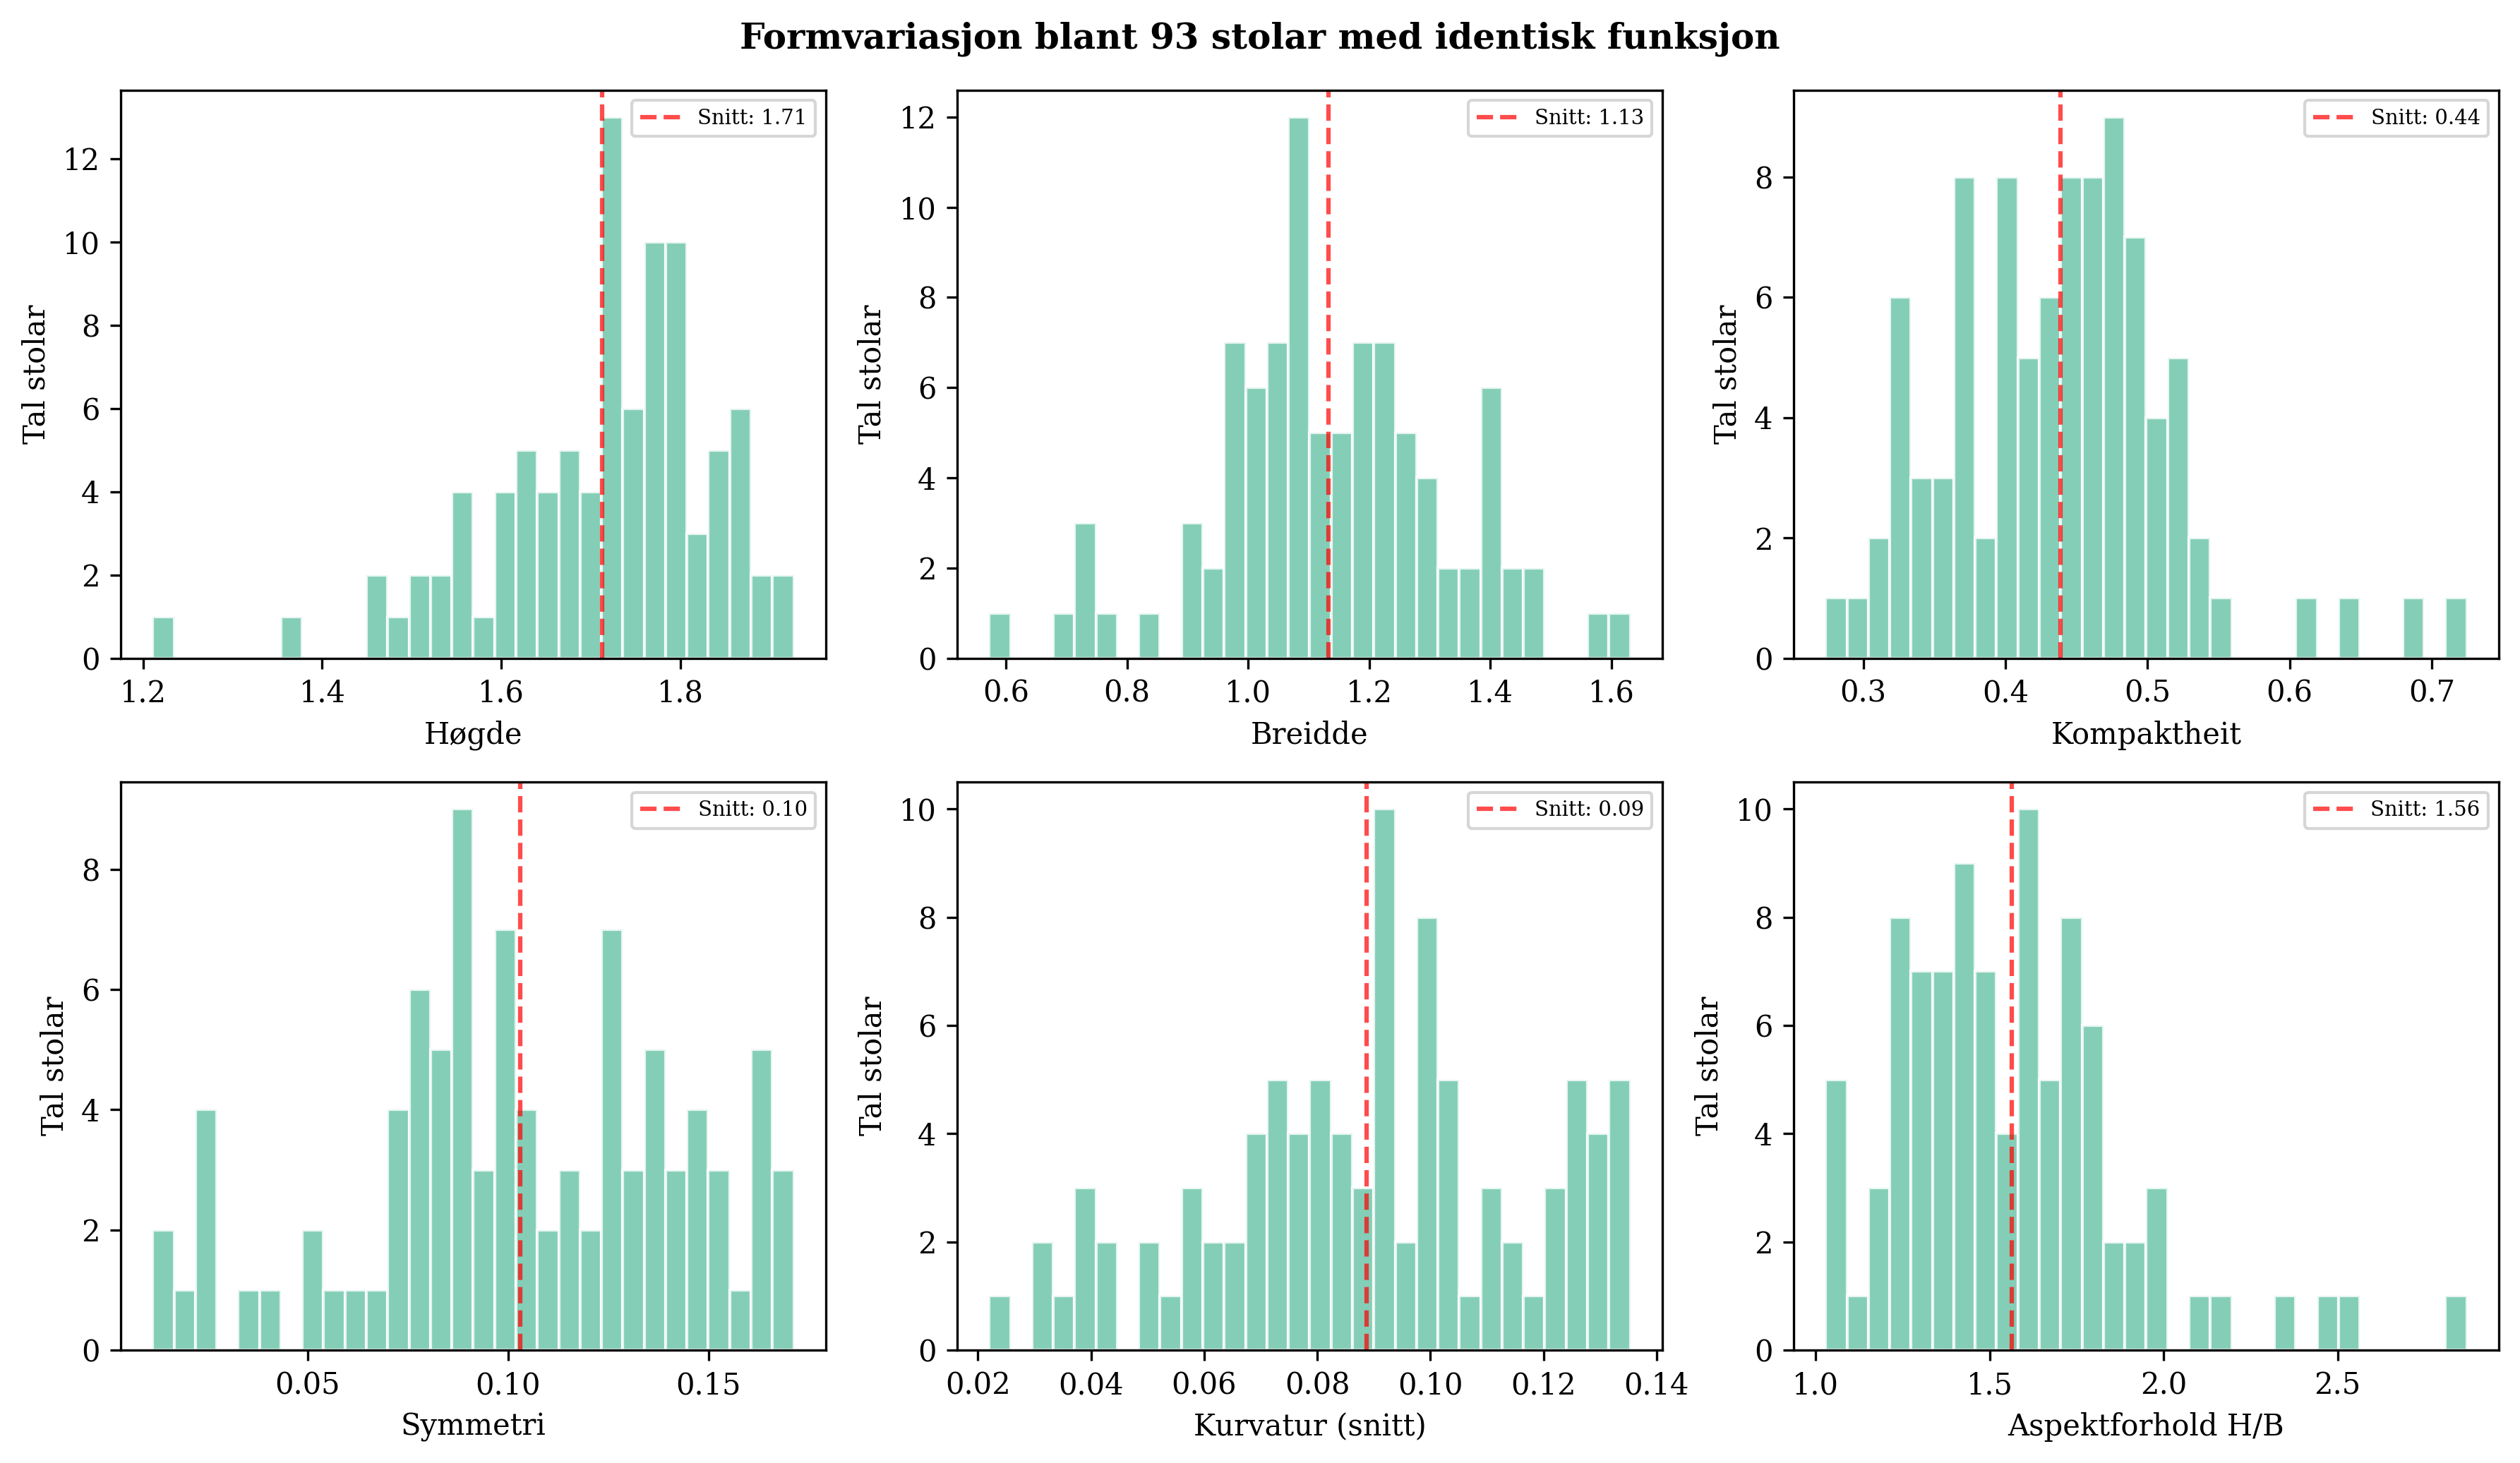
\includegraphics[width=\textwidth]{figurar/fig1_form_variasjon.png}
\caption{Distribusjon av seks geometriske eigenskapar for 93~stolar med identisk funksjon. R\o{}d stipla linje markerer gjennomsnitt. Den breie spreiinga viser at funksjon ikkje avgjer form.}
\label{fig:formvariasjon}
\end{figure}

% ---- Bevis II ----
\subsection{Bevis II: Material predikerer form}
\label{sec:bevis2}

Me testar den f\o{}rste alternative hypotesen: at \emph{materialval} er ein sterkare formgjevar enn funksjon. For kvart av dei 30~materiala og kvar av dei 21~geometriske eigenskapane utf\o{}rer me ein Mann--Whitney $U$-test med Bonferroni-korreksjon. Tabell~\ref{tab:materialform} viser dei st\o{}rste effektane.

\begin{table}[H]
\centering
\caption{Topp 10 material$\rightarrow$form-koplingar (Cohens $d$)}
\label{tab:materialform}
\begin{tabular}{llcc}
\toprule
\textbf{Material} & \textbf{Geometrisk eigenskap} & \textbf{Cohens $d$} & $n$ \\
\midrule
Ull & D2-bin 4 (formfordeling) & 1.60 & 10 \\
Metall & H\o{}gde (bbox\_H) & 1.47 & 6 \\
Skumplast & H\o{}gdefordeling midt & 1.40 & 14 \\
Gummi/plast & D2-bin 4 & 1.39 & 5 \\
Gummi/plast & D2-bin 5 & 1.35 & 5 \\
Ull & H\o{}gdefordeling midt & 1.31 & 10 \\
Skumplast & H\o{}gdefordeling botn & 1.29 & 14 \\
Ull & D2-bin 2 & 1.28 & 10 \\
Skumplast & D2-bin 4 & 1.26 & 14 \\
Mahogni & H\o{}gde (bbox\_H) & 1.20 & 6 \\
\bottomrule
\end{tabular}
\end{table}

\noindent
Effektstorleikane er sv\ae{}rt store ($d > 1.0$). At ull, skumplast og gummi dominerer topplista avspeglar det industrielle skiftet: polstra stolar har ein fundamentalt annleis massefordeling enn reine trekonstruksjonar. Materialet \emph{tvingar} forma.

\begin{figure}[H]
\centering
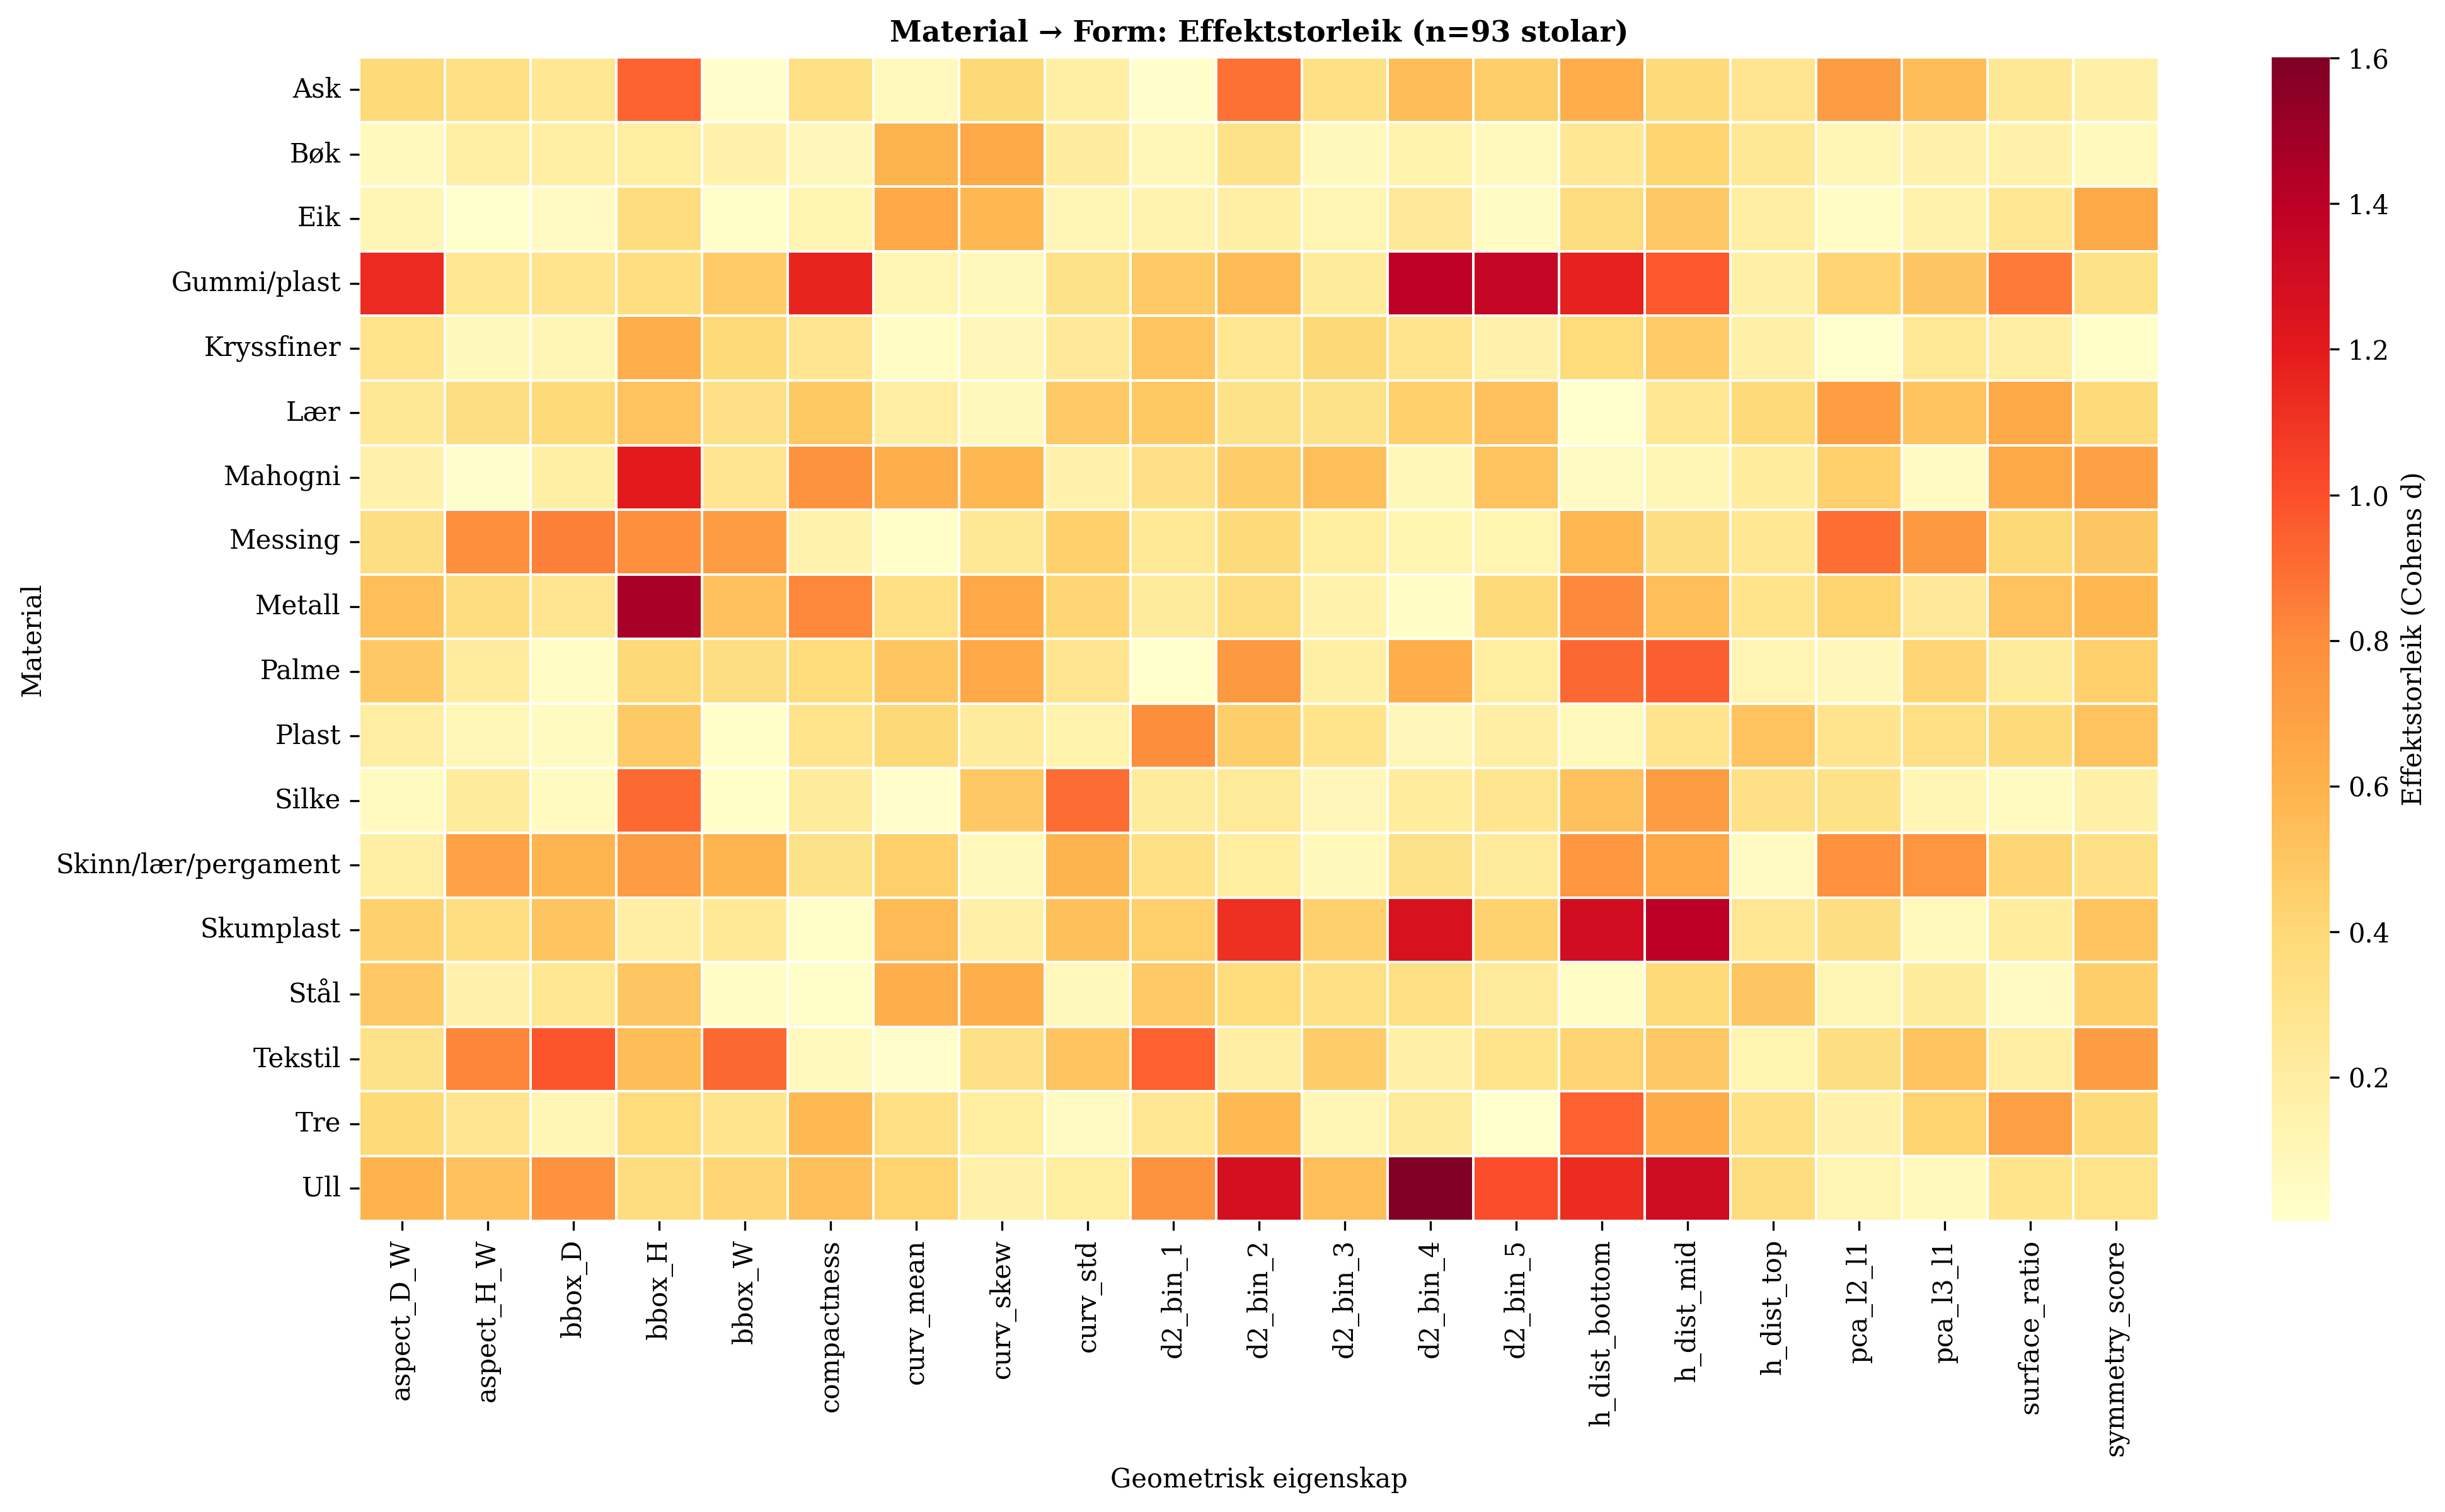
\includegraphics[width=\textwidth]{figurar/fig2_material_form_heatmap.png}
\caption{Varmekart over effektstorleik (Cohens $d$) for material--geometri-koplingar. Kvart material definerer ein distinkt geometrisk profil.}
\label{fig:heatmap}
\end{figure}

% ---- Bevis III ----
\subsection{Bevis III: Materialaffordanse som geometrisk signatur}
\label{sec:bevis3}

\citet{gibson1977} definerte affordanse som handlingane eit milj\o{} tilbyr ein akt\o{}r. Her ser me at kvart material tilbyr ei distinkt formverd (Tabell~\ref{tab:affordance}).

\begin{table}[H]
\centering
\caption{Geometrisk profil per hovudmaterial (snitt $\pm$ standardavvik)}
\label{tab:affordance}
\begin{tabular}{lccccc}
\toprule
\textbf{Material} & $n$ & \textbf{Kompaktheit} & \textbf{Symmetri} & \textbf{Kurvatur} & \textbf{Aspekt H/B} \\
\midrule
Mahogni & 6 & 0.381 & 0.129 & 0.105 & 1.57 \\
Eik & 22 & 0.447 & 0.123 & 0.103 & 1.57 \\
B\o{}k & 21 & 0.445 & 0.101 & 0.101 & 1.61 \\
Kryssfiner & 27 & 0.455 & 0.104 & 0.090 & 1.58 \\
St\aa{}l & 20 & 0.437 & 0.118 & 0.075 & 1.52 \\
\bottomrule
\end{tabular}
\end{table}

\noindent
Mahognistolar er minst kompakte (0.381): materialet sin h\o{}ge brotstyrke let formgjevaren spreie massen ut i slankare lemer. St\aa{}lstolar har l\aa{}gast kurvatur (0.075): metallet sitt formspr\aa{}k tenderer mot rette linjer. Kryssfiner gjev h\o{}gast kompaktheit (0.455): det laminerte materialet inviterer til kontursty\-rande skalformer. Materialet legg l\o{}ynde stiar i fitnesskartet \citep{pye1968, gibson1977}.

\begin{figure}[H]
\centering
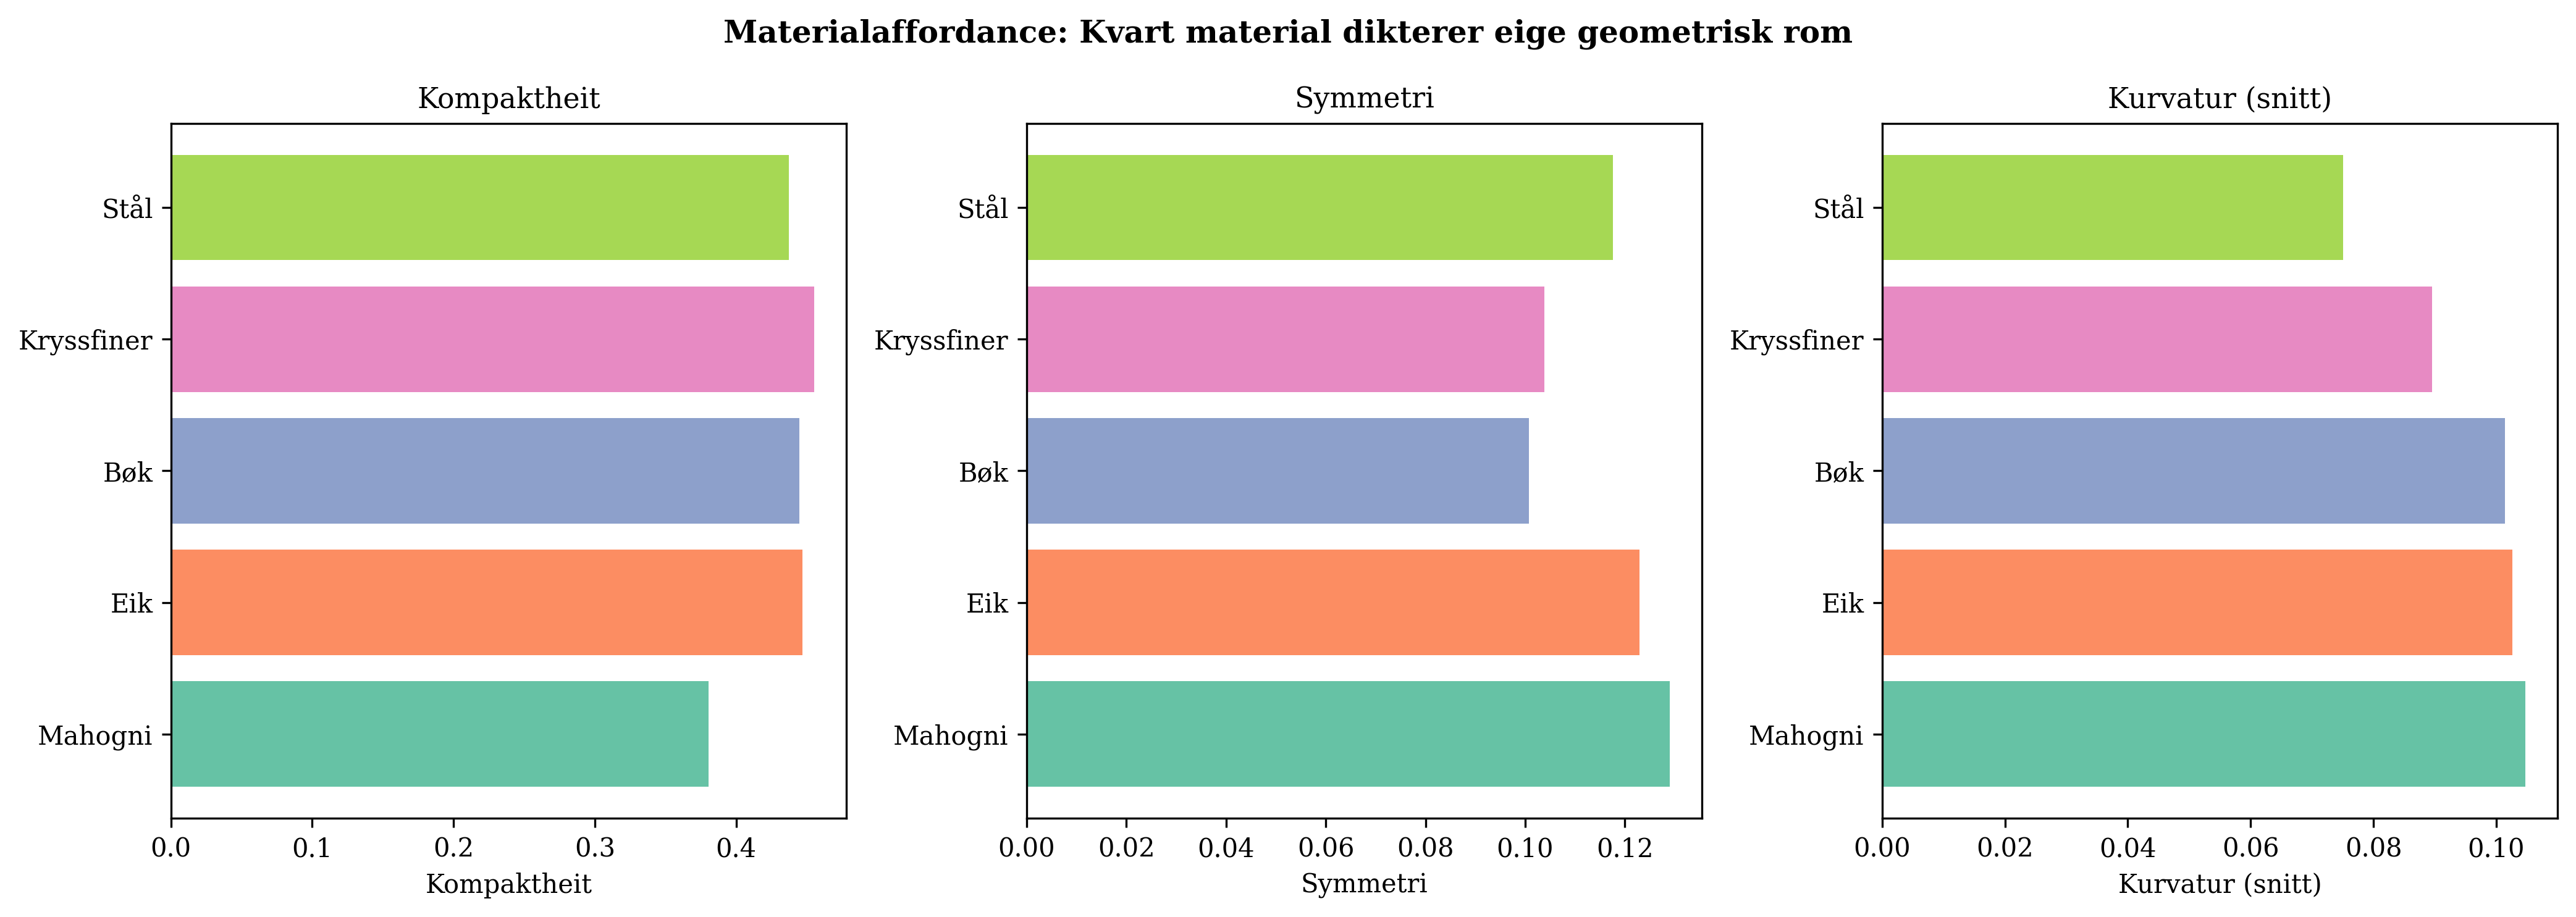
\includegraphics[width=\textwidth]{figurar/fig5_material_affordance.png}
\caption{Materialaffordanse: kvar materialgruppe okkuperer ein distinkt del av det geometriske rommet. Profilane er ikkje styrt av funksjon (som er identisk), men av materialet si innebygde yteevne.}
\label{fig:affordance}
\end{figure}

% ---- Bevis IV ----
\subsection{Bevis IV: Fitnesslandskapet i informasjonsteoretisk dekomponering}
\label{sec:bevis4}

Me nyttar \emph{mutual information} (MI) for \aa{} kvantifisere kor mykje kvar seleksjonsfaktor fortel om geometrisk form \citep{cover2006}. For kvar av 21~geometriske eigenskapar (diskretisert i kvintilgrupper) reknar me MI mot tre kategoriske seleksjonstrykk:

\begin{table}[H]
\centering
\caption{Gjennomsnittleg mutual information mellom seleksjonstrykk og form}
\label{tab:mi}
\begin{tabular}{lcc}
\toprule
\textbf{Seleksjonstrykk} & \textbf{Snitt MI (bits)} & \textbf{Relativ styrke} \\
\midrule
Material & 0.382 & 1.00 \\
Tid (hundre\aa{}r) & 0.168 & 0.44 \\
Geografi (opphav) & 0.079 & 0.21 \\
\bottomrule
\end{tabular}
\end{table}

\noindent
Material ber \emph{fem gonger} meir informasjon om form enn geografi. Tidsperioden ligg mellom, noko som gjev meining fordi materialtilgang endrar seg over tid. Funksjon er ikkje med i tabellen: den er per definisjon konstant ($\mathrm{MI_{funksjon}} = 0$).

PCA p\aa{} det kombinerte 51-dimensjonale featurerommet viser at dei tre f\o{}rste komponentane forklarer 33.8\,\% av variansen (PC1: 14.0\,\%, PC2: 11.8\,\%, PC3: 7.9\,\%). At ingen einskild komponent dominerer, stadfester det fleirdimensjonale i fitnesslandskapet.

\begin{figure}[H]
\centering
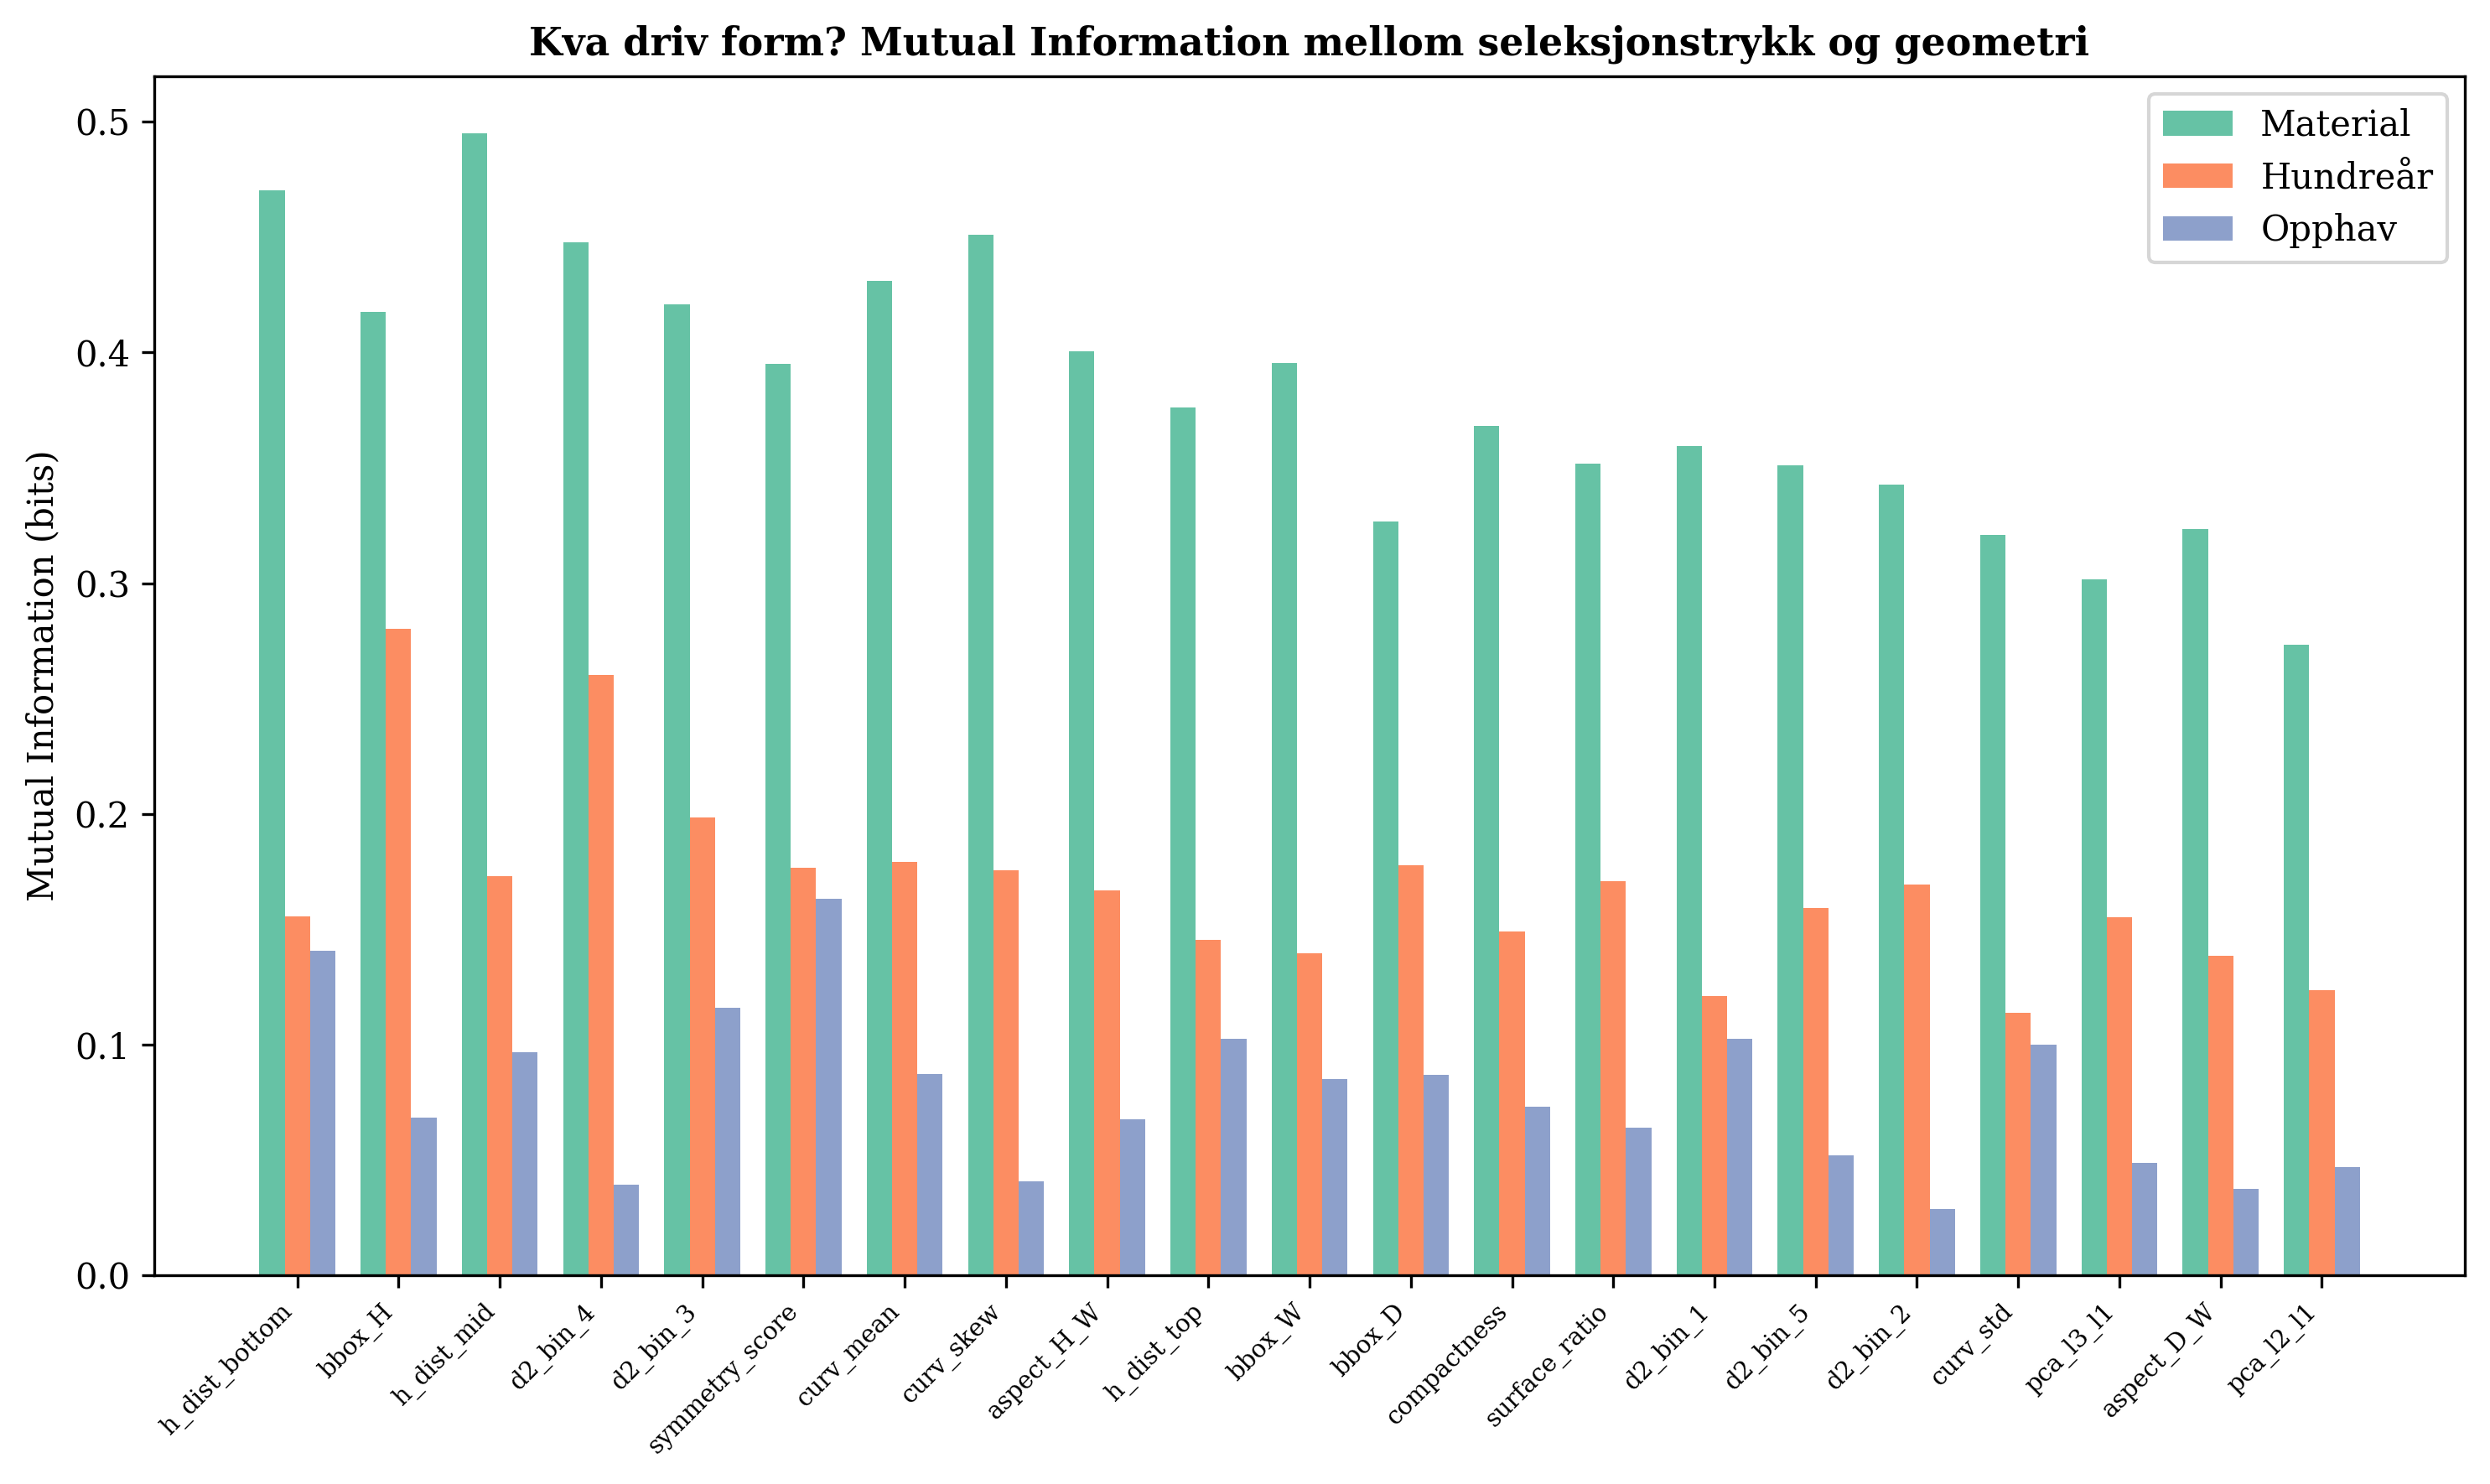
\includegraphics[width=\textwidth]{figurar/fig6_mutual_information.png}
\caption{Mutual information per geometrisk eigenskap. Bl\aa{}: material, oransje: tid, gr\o{}n: geografi. Material dominerer p\aa{} tvers av nesten alle eigenskapar.}
\label{fig:mi}
\end{figure}

\begin{figure}[H]
\centering
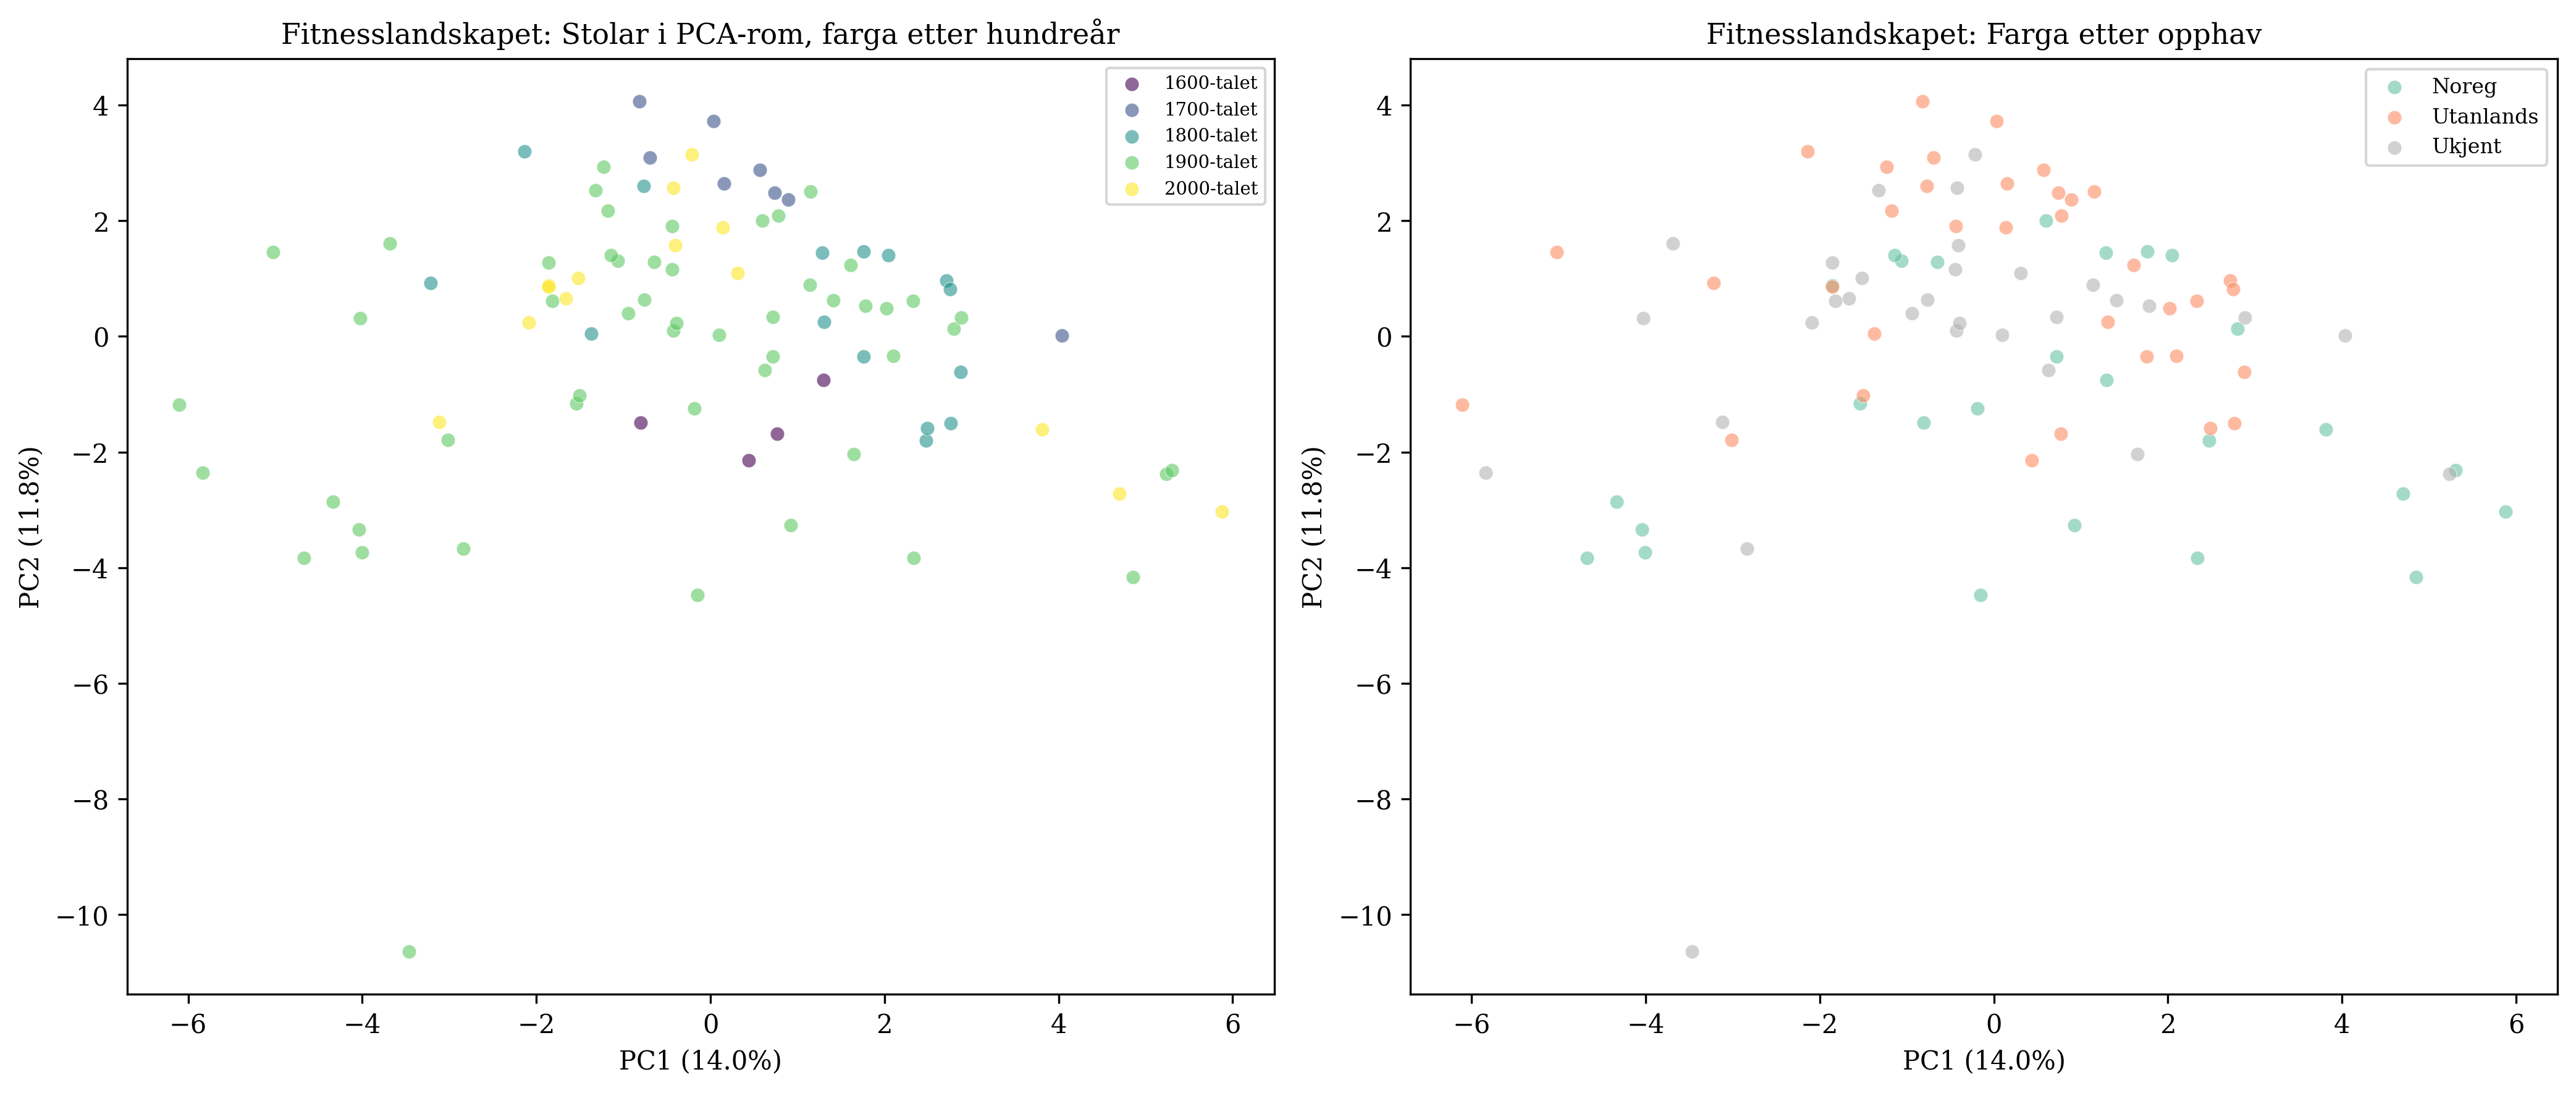
\includegraphics[width=\textwidth]{figurar/fig3_fitness_landscape_pca.png}
\caption{Fitnesslandskapet i PCA-rom. \textbf{Venstre}: Farga etter hundre\aa{}r. Tidsperiodane okkuperer ulike regionar, noko som viser at landskapet skiftar over tid. \textbf{H\o{}gre}: Farga etter opphav (Noreg vs.\ utland).}
\label{fig:pca}
\end{figure}

% ---- Bevis V ----
\subsection{Bevis V: Stil er emergent, ikkje kausal}
\label{sec:bevis5}

Er stilkategoriane \emph{kausale} (dei driv form), eller \emph{emergente} (dei er eit etterskot)? Me testar dette med Random Forest-prediksjon av geometriske formklynger ($K$-means $k = 6$, 5-fold CV).

\begin{table}[H]
\centering
\caption{Random Forest-prediksjon av formklynger fr\aa{} ulike prediktorsett}
\label{tab:prediction}
\begin{tabular}{lcc}
\toprule
\textbf{Prediktorsett} & \textbf{$F_1$ (makro)} & $\pm$ \textbf{std} \\
\midrule
Berre stilperiode & 0.186 & 0.122 \\
Berre material (30 var.) & 0.334 & 0.108 \\
Berre tid (\aa{}rstal) & 0.438 & 0.088 \\
Material + tid & 0.401 & 0.084 \\
Material + tid + opphav & 0.383 & 0.103 \\
\bottomrule
\end{tabular}
\end{table}

\noindent
\textbf{Stilperiode ($F_1 = 0.19$) predikerer form d\aa{}rlegast av alle alternativ.} Tid ($F_1 = 0.44$) og material ($F_1 = 0.33$) sl\aa{}r stilmerkelappen kvar for seg. Stilkategoriane er s\aa{}leis ikkje kausale mekanismar, men emergente merkelappar \citep{boyd1985}. Stil er eit \emph{symptom}, ikkje ein \emph{\aa{}rsak}.

% ---- Bevis VI ----
\subsection{Bevis VI: Exploration- og exploitation-syklusar}
\label{sec:bevis6}

I reinforcement learning vekslar ein agent mellom exploration og exploitation \citep{sutton2018}. Dersom FFF held, b\o{}r me sj\aa{} tilsvarande syklusar i designhistoria. Me m\aa{}ler formdiversitet som gjennomsnittleg parvis euklidisk avstand i det standardiserte 21-dimensjonale geometrirommet per 50-\aa{}rsperiode:

\begin{table}[H]
\centering
\caption{Formdiversitet per 50-\aa{}rsperiode}
\label{tab:diversity}
\begin{tabular}{lccc}
\toprule
\textbf{Periode} & $n$ & \textbf{Formdiversitet} & \textbf{Fase} \\
\midrule
1600--1649 & 3 & 1.83 & L\aa{}g (f\o{}r-kolonialt) \\
1750--1799 & 7 & 3.16 & Stigande \\
1850--1899 & 15 & 4.34 & Industriell exploration \\
1900--1949 & 10 & 5.60 & H\o{}g (materialeksplosjon) \\
1950--1999 & 42 & 6.97 & Topp (postmoderne) \\
2000--2049 & 14 & 6.46 & Konsolidering? \\
\bottomrule
\end{tabular}
\end{table}

\noindent
Formdiversiteten aukar monotont fr\aa{} 1.83 (1600-talet) til 6.97 (1950--1999). Men den \emph{synk} att til 6.46 etter 2000, eit mogleg signal om at det postmoderne eksperimentet no er i ein exploitation-fase. Denne dynamikken samsvarar med mønsteret \citet{gould1972} skildra i paleobiologien: langvarig stase avbroten av braa endringar.

\begin{figure}[H]
\centering
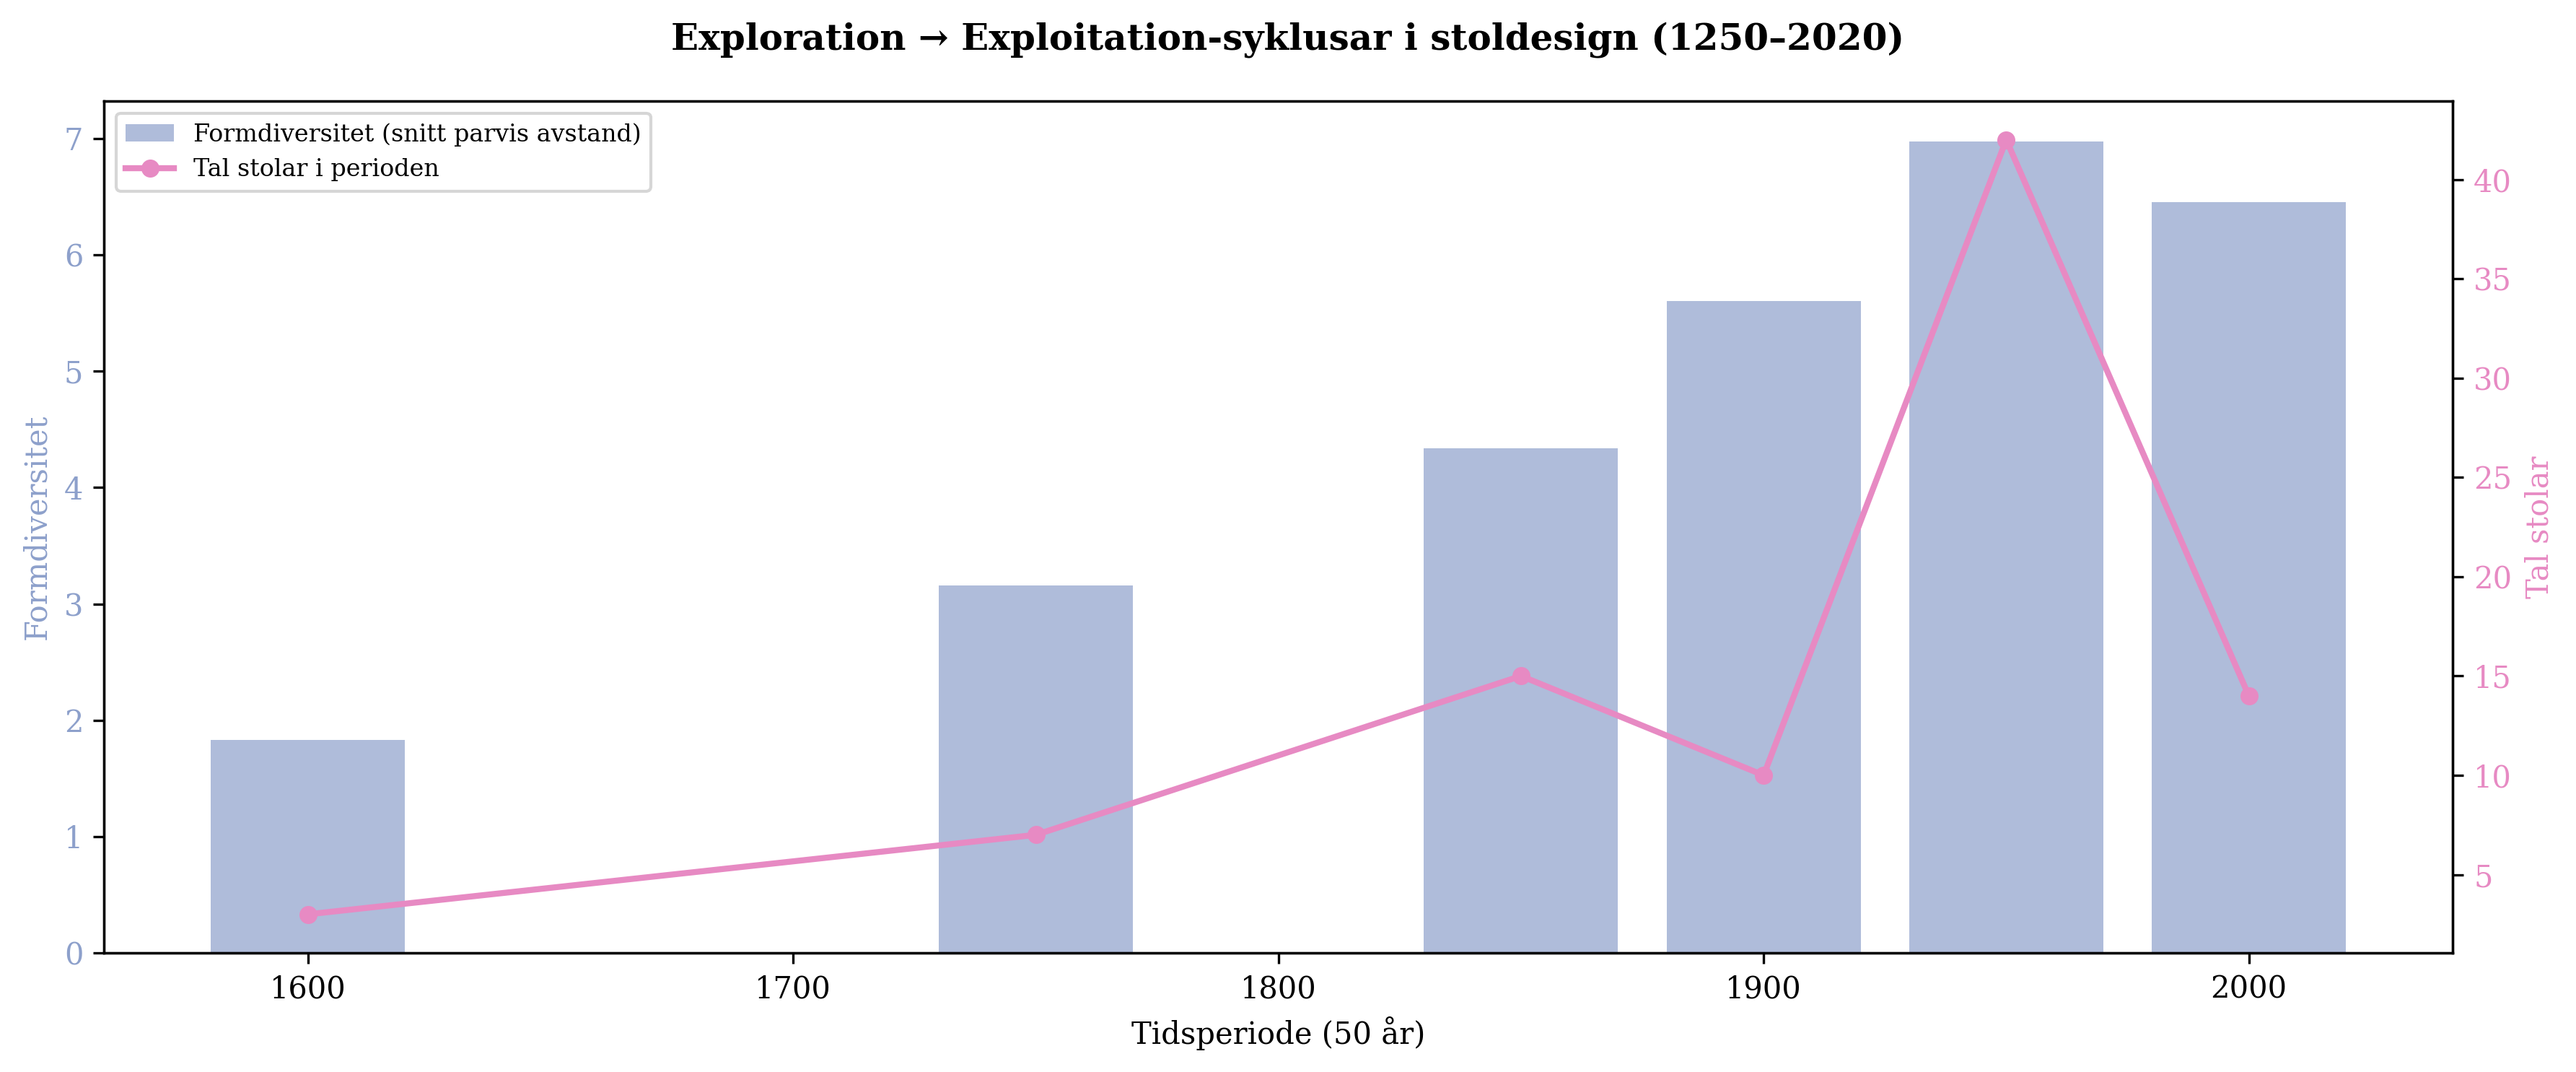
\includegraphics[width=\textwidth]{figurar/fig4_exploration_exploitation.png}
\caption{Formdiversitet (bl\aa{} bar) og tal stolar (oransje linje) per 50-\aa{}rsperiode. Aukande diversitet avspeglar fleire tilgjengelege materiale og produksjonsmetodar, eit rikare fitnesslandskap.}
\label{fig:expexpl}
\end{figure}

% ---- Bevis VII ----
\subsection{Bevis VII: Temporal drift i fitnesslandskapet}
\label{sec:bevis7}

Dersom fitnesslandskapet var statisk, ville stolar fr\aa{} ulike tider likne kvarandre i same grad. Me m\aa{}ler drift som euklidisk avstand mellom periodane sine sentroidar i standardisert geometrirom:

\begin{table}[H]
\centering
\caption{Drift mellom 50-\aa{}rsperiodar (euklidisk avstand, standardisert rom)}
\label{tab:drift}
\begin{tabular}{lcc}
\toprule
\textbf{Overgang} & \textbf{Drift} & \textbf{Historisk kontekst} \\
\midrule
1600 $\rightarrow$ 1750 & 11.66 & Koloniale materiale kjem \\
1750 $\rightarrow$ 1850 & 7.24 & Mahognitoppen \\
1850 $\rightarrow$ 1900 & 3.93 & Industriell standardisering \\
1900 $\rightarrow$ 1950 & 5.13 & Nye syntetiske materiale \\
1950 $\rightarrow$ 2000 & 4.75 & Postmodernistisk pluralisme \\
\bottomrule
\end{tabular}
\end{table}

\noindent
Den desidert st\o{}rste drifta (11.66) fell mellom 1600-talet og 1750, \emph{nett n\aa{}r koloniale materialar vert tilgjengelege i Noreg} \citep{finne2026a}. Innf\o{}rsla av nytt material la ikkje berre til fleire formar, men forskyvde heile tyngdepunktet i fitnesslandskapet. Denne temporale drifta er det st\o{}rste empiriske argumentet mot \enquote{form follows function}: funksjonen \enquote{sitte p\aa{}} har ikkje endra seg p\aa{} 400~\aa{}r, men fitnesslandskapet har skifta dramatisk, og forma har fylgd.

\begin{figure}[H]
\centering
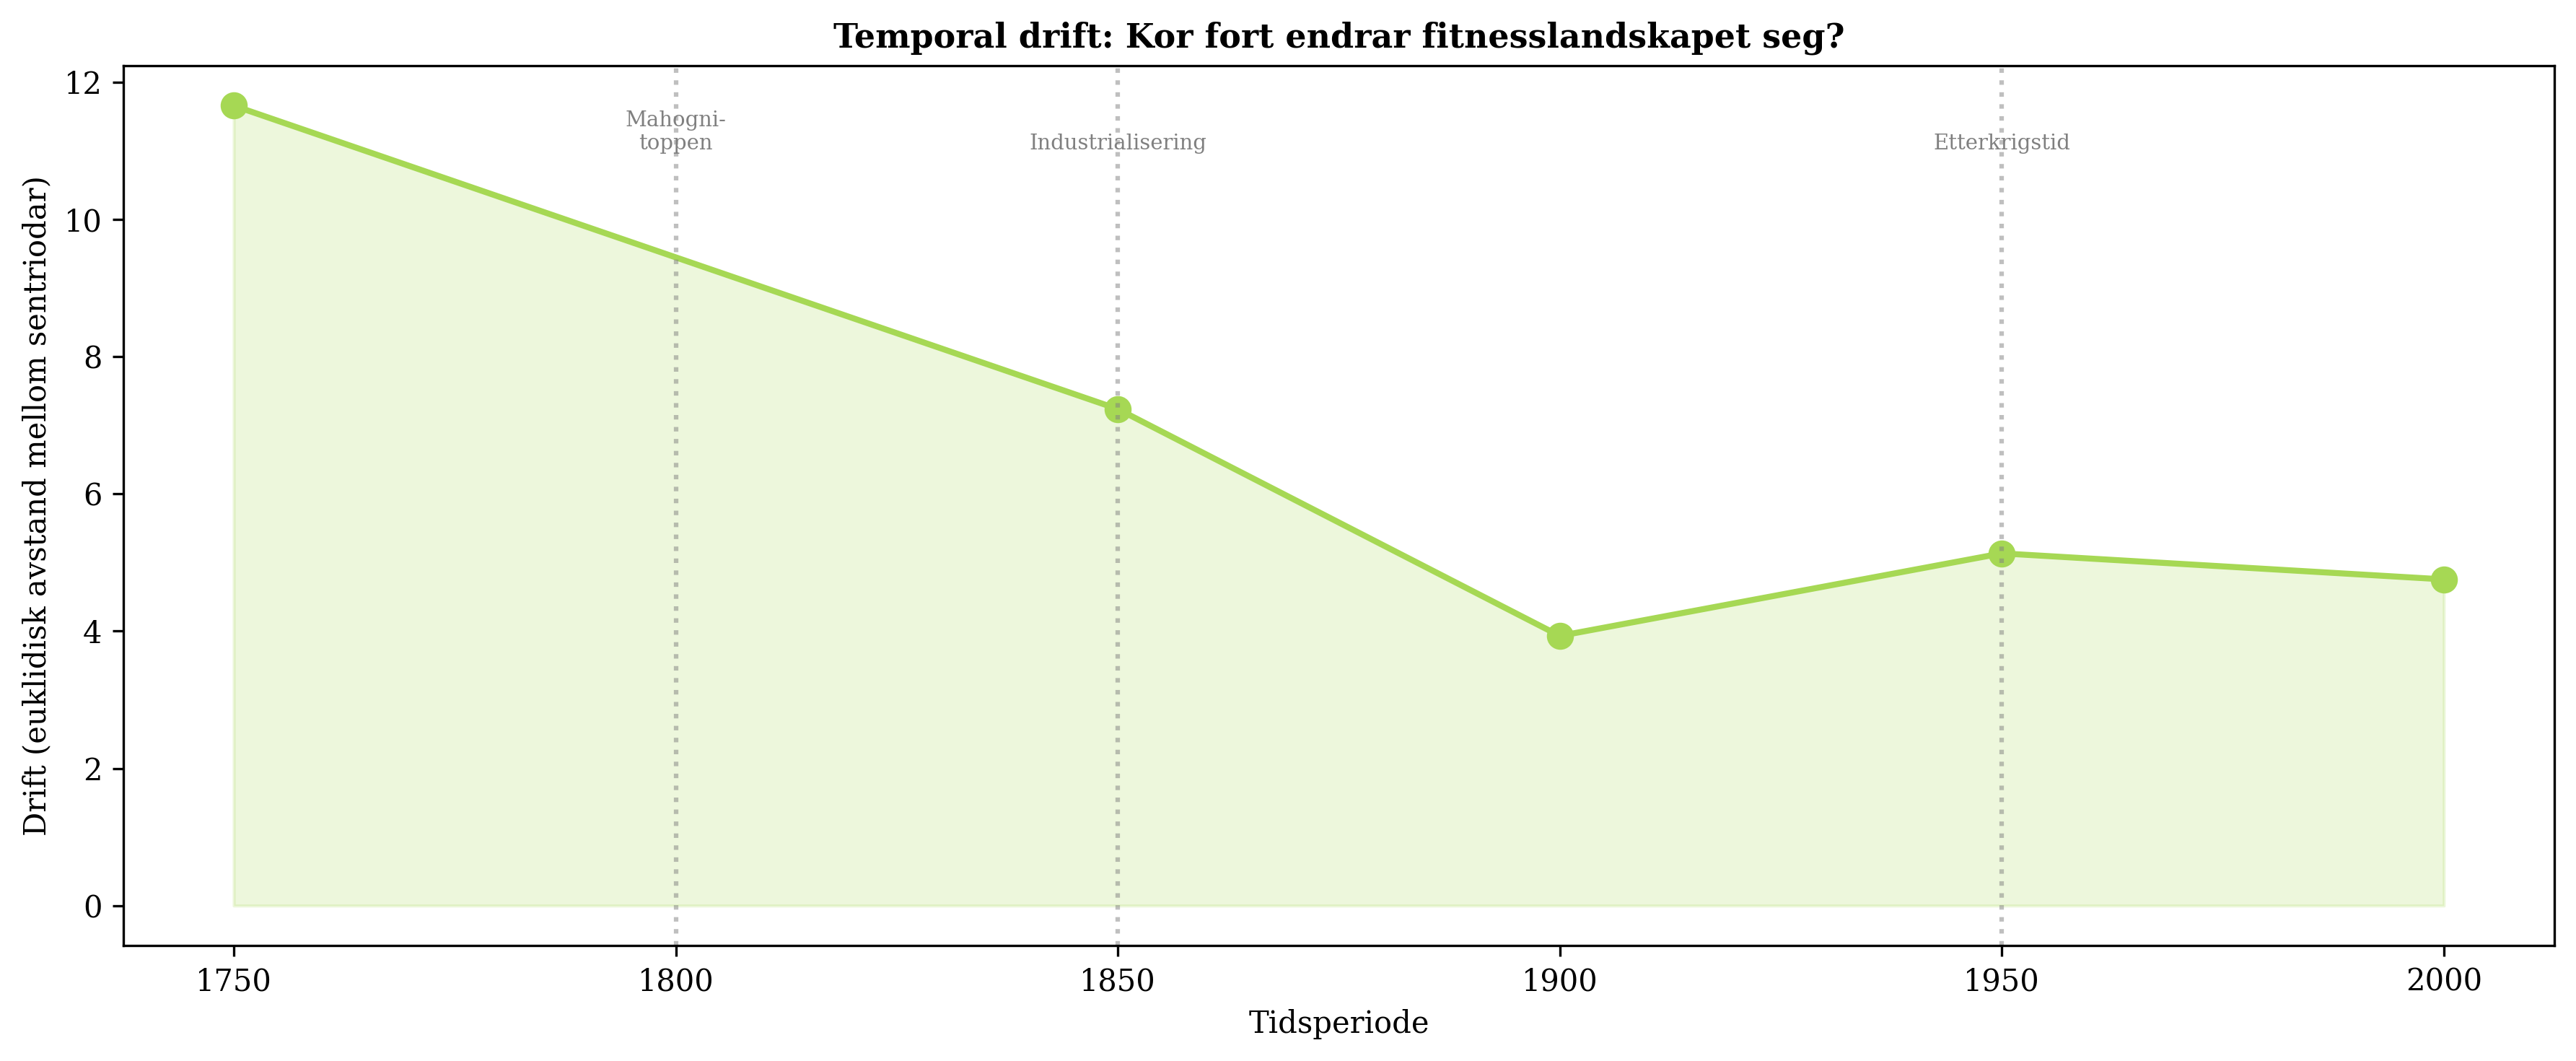
\includegraphics[width=\textwidth]{figurar/fig7_temporal_drift.png}
\caption{Temporal drift i fitnesslandskapet. Toppunktet mellom 1600 og 1750 samanfell med innf\o{}rsla av koloniale materiale.}
\label{fig:drift}
\end{figure}

% ---- Bevis VIII ----
\subsection{Bevis VIII: Materialentropi og politiske sjokk}
\label{sec:bevis8}

Shannon-entropien i materialfordelinga gjev eit m\aa{}l p\aa{} kor \enquote{flatt} eller \enquote{spiss} materiallandskapet er i ein gjeven periode. H\o{}g entropi t\ae{}ler for mange ulike materiale i bruk (exploration); l\aa{}g entropi t\ae{}ler for dominans av eitt material (exploitation).

\begin{table}[H]
\centering
\caption{Shannon-entropi i materialfordelinga per periode}
\label{tab:entropy}
\begin{tabular}{lccc}
\toprule
\textbf{Periode} & $n$ & \textbf{Entropi (bits)} & \textbf{Materialar i bruk} \\
\midrule
1600-talet & 3 & 2.50 & 6 \\
1750-talet & 7 & 1.50 & 3 \\
1850-talet & 15 & 3.33 & 13 \\
1900-talet & 10 & 2.47 & 7 \\
1950-talet & 42 & 3.49 & 17 \\
2000-talet & 14 & 3.26 & 12 \\
\bottomrule
\end{tabular}
\end{table}

\noindent
Entropien kollapsar fr\aa{} 2.50 til 1.50~bit mellom 1600 og 1750. Dette er \emph{mahognitoppen}: eitt kolonimaterial dominerer s\aa{} sterkt at det utkonkurrerer alle alternativ. Samlinga g\aa{}r fr\aa{} seks til tre materiale i bruk. Dette er klassisk exploitation \citep{sutton2018}: ein fitness-topp s\aa{} dominant at heile systemet konvergerer mot \'{e}in l\o{}ysing. Industrialiseringa (1850) knuser dette monopolet og dyttar entropien til 3.33~bit, 13 materiale i bruk. Nye produksjonsmetodar gjer fleire materiale \emph{fit}, og systemet g\aa{}r inn i ein ny exploration-fase.

\begin{figure}[H]
\centering
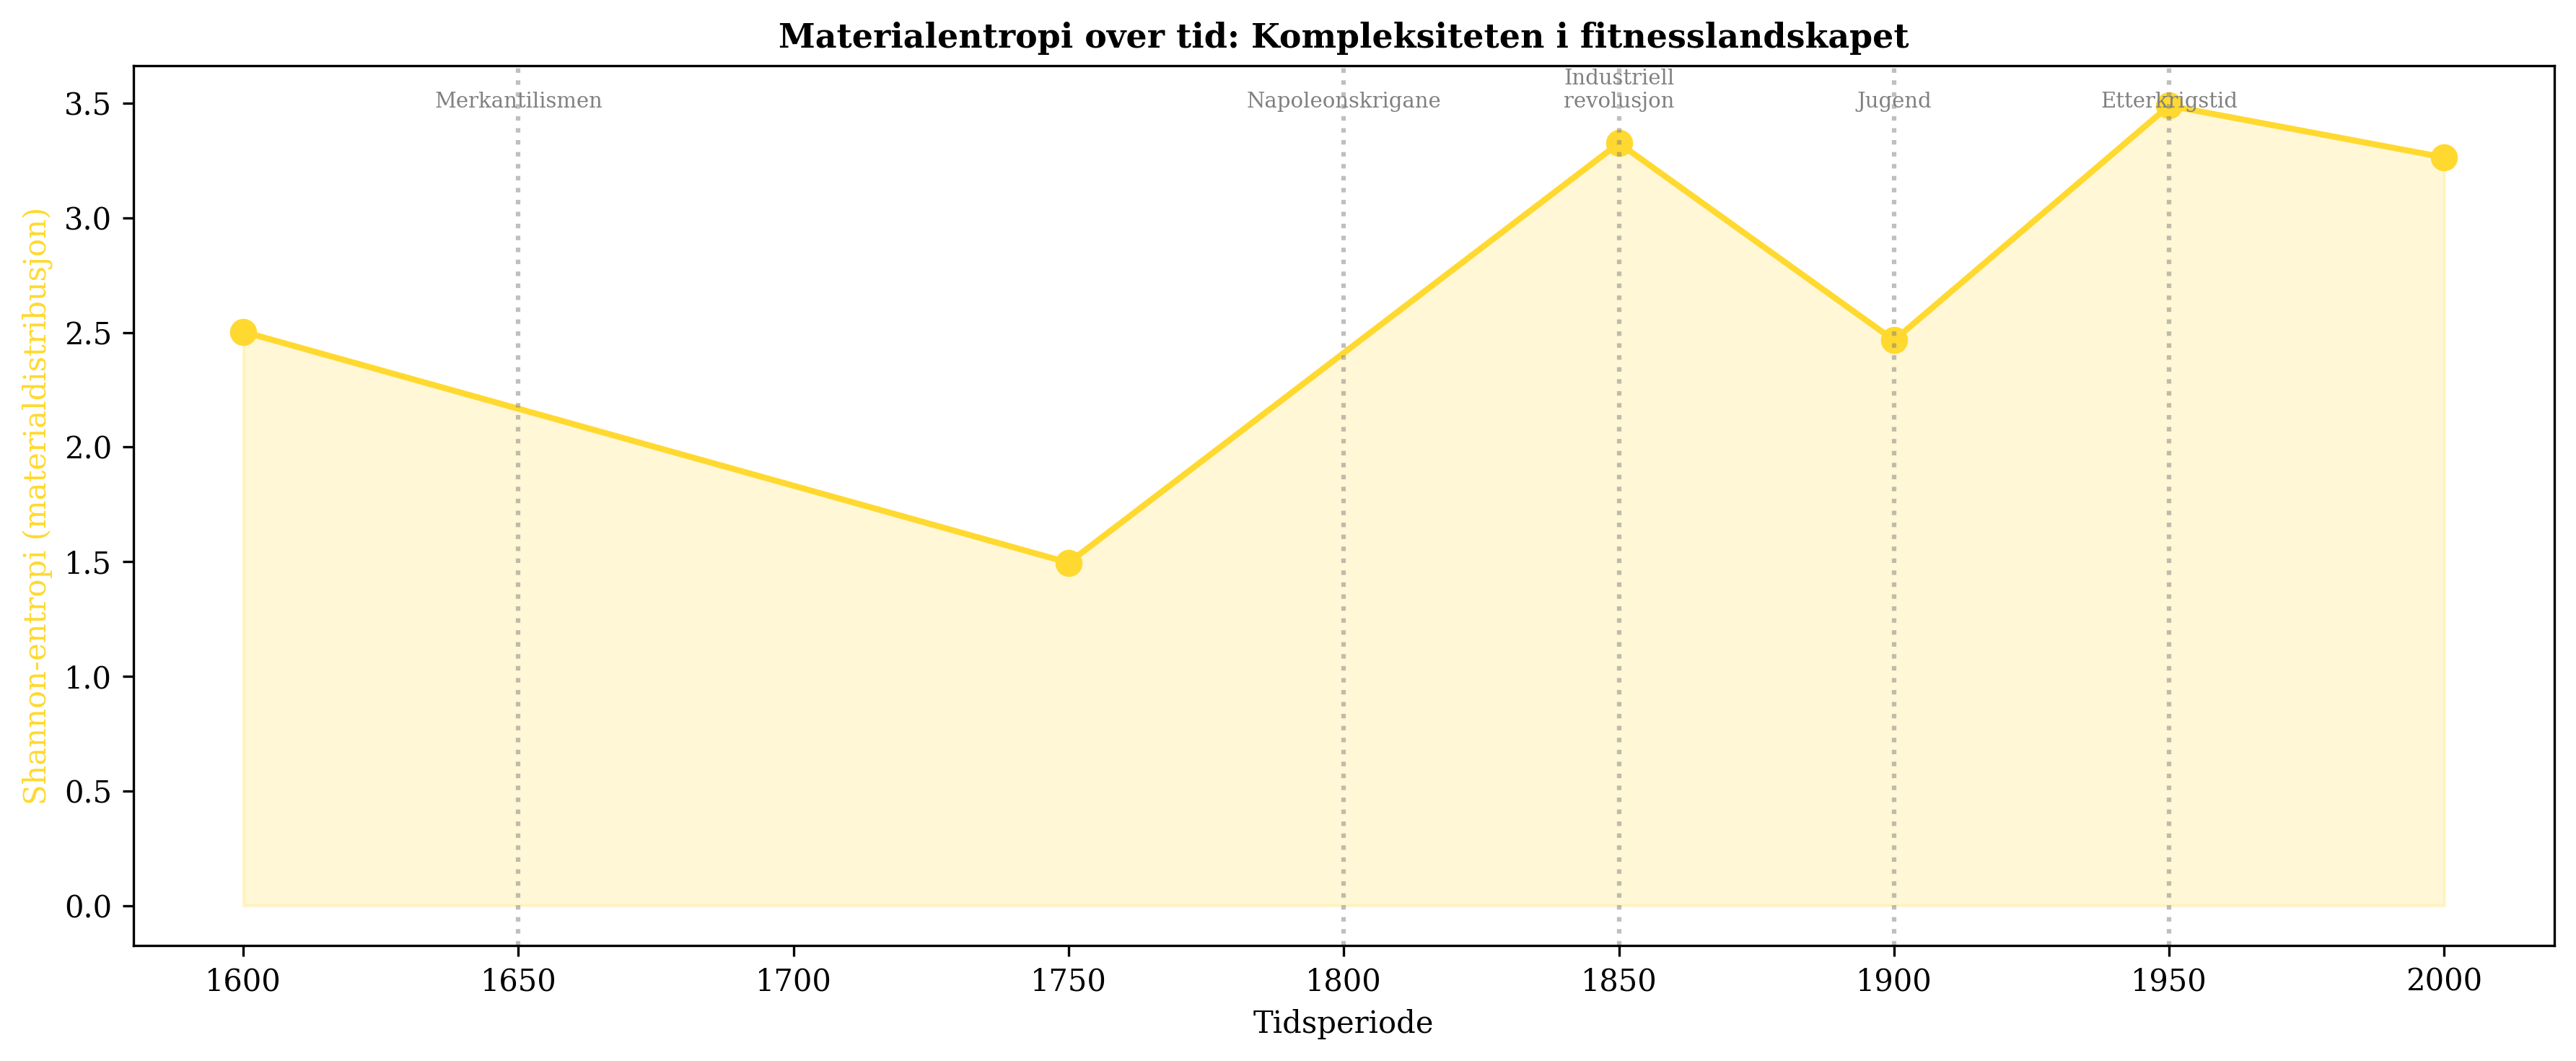
\includegraphics[width=\textwidth]{figurar/fig9_material_entropy.png}
\caption{Shannon-entropi i materialfordelinga over tid. Kollapsen p\aa{} 1750-talet avspeglar mahognien si dominans; den industrielle revolusjonen (1850) opnar for eit nytt, rikare materiallandskap.}
\label{fig:entropy}
\end{figure}

% -------------------------------------------------------------------
\section{Syntese: Dei tre f\o{}rste artiklane i lys av fitnesskartet}
\label{sec:syntese}

Det empiriske grunnlaget i seksjonane ovanfor let oss refortolke funna fr\aa{} dei tre f\o{}reg\aa{}ande artiklane, ikkje som isolerte observasjonar, men som manifestasjonar av same underliggjande dynamikk.

\subsection{Art.~I: Mahogniens boge som topografisk kollaps}

\citet{finne2026a} dokumenterte korleis mahognibruk f\o{}lgde ei boge fr\aa{} 23\,\% (1775) til 86\,\% (1825) og tilbake til 4\,\% (1900). Bevis~VIII viser no at denne bogen kollapsa materialentropien fr\aa{} 2.5 til 1.5~bit. I FFF-terminologi: mahogni sin kombinasjon av h\o{}g brotstyrke, let bearbeidbarheit og kolonialt prestisjesignal \citep{zahavi1975} skapte ein s\aa{} kraftig fitness-topp at heile designlandskapet konvergerte, ein klassisk exploitation-syklus.

\subsection{Art.~II: Stilmigrasjon som driftm\o{}nster}

\citet{finne2026b} viste korleis stilar migrerer og konvergerer over tid. Bevis~VII kvantifiserer no denne migrasjonen som drift mellom sentroidar. Den st\o{}rste drifta (11.66) fell saman med innf\o{}rsla av koloniale materiale. Stilmigrasjonen er s\aa{}leis ikkje eit sj\o{}lvstendig fenomen, men ein konsekvens av at fitnesslandskapet skiftar underflata \citep{odlingsmee2003}. N\aa{}r nye materiale kjem, trekk dei formsentroidane med seg.

\subsection{Art.~III: 3D-form som fitnessindikator}

\citet{finne2026c} viste at 3D-geometri ber informasjon om b\aa{}de nasjonalitet og tidsalder. Bevis~IV stadfester dette: den kumulative PCA-variansen (33.8\,\% i tre komponentar) og den monotont aukande formdiversiteten demonstrerer at geometrien kodar eit rikt informasjonslager. Formrommet er eit fitnesskart i 21~dimensjonar.

% -------------------------------------------------------------------
\section{Diskusjon}
\label{sec:diskusjon}

\subsection{Kva FFF er}

\emph{Form Follows Fitness} er eit rammeverk der form vert forst\aa{}tt som \emph{selektert}, ikkje dedusert. Forma p\aa{} ein stol er ikkje eit logisk svar p\aa{} sp\o{}rsm\aa{}let \enquote{korleis sit ein best?}, men eit mellombels optimum i eit fleirdimensjonalt landskap \citep{wright1932, kauffman1993} definert av:

\begin{enumerate}[nosep]
    \item \textbf{Materialaffordanse} (MI = 0.382): Det st\o{}rste einskildtrykket.
    \item \textbf{Temporalt trykk} (MI = 0.168): Teknologi, \o{}konomi og politikk skiftar landskapet.
    \item \textbf{Geografisk trykk} (MI = 0.079): Lokal materialtilgang skapar regionale optimum.
    \item \textbf{Funksjon} (MI = 0): Eit hygienekrav, ikkje ein formgjevar.
\end{enumerate}

\subsection{Kva FFF ikkje er}

FFF p\aa{}st\aa{}r ikkje at funksjon er uviktig. Ein stol m\aa{} b\ae{}re ein kropp. Men dette kravet er s\aa{} basalt, og s\aa{} overbestemt av materialets eigne eigenskapar, at det i praksis ikkje avgrensar formrommet. Funksjon er eit \emph{n\o{}dvendig} vilk\aa{}r, men ikkje eit \emph{tilstrekkjeleg} vilk\aa{}r for \aa{} forklare form. FFF er heller ikkje biologisk determinisme: me nyttar evolusjon\ae{}re modellar som \emph{analogiar}, ikkje som \aa{}rsakskoplingar \citep{henrich2016}.

\subsection{Sullivan og Le~Corbusier som spesialtilfelle}

\enquote{Form follows function} er gyldig n\aa{}r alle andre seleksjonstrykk er noytraliserte. Dette er eit \emph{degenerert spesialtilfelle} som aldri eksisterer i praksis, fordi materialtilgang, \o{}konomiske vilk\aa{}r og kulturelle preferansar alltid utover trykk. FFF generaliserer funksjonalismen: Sullivan og Le~Corbusier sine prinsipp er spesialtilfelle der $\mathrm{MI_{material}} = \mathrm{MI_{tid}} = \mathrm{MI_{geografi}} = 0$, og berre funksjon st\aa{}r att. V\aa{}re data viser at dette vilk\aa{}ret aldri er oppfylt.

\subsection{Implikasjonar for designpraksis}

Dersom form ikkje f\o{}lgjer funksjon, men fitness, endrar det korleis me underviser og praktiserer design:

\begin{itemize}[nosep]
    \item \textbf{Materialval f\o{}rst}: Designprosessen b\o{}r starte med materialets affordanse, ikkje med eit funksjonskravsdokument.
    \item \textbf{Seleksjonstrykk som designverkt\o{}y}: I staden for \aa{} sp\o{}rje \enquote{kva er funksjonen?}, b\o{}r designaren sp\o{}rje \enquote{kva er seleksjonstrykka?}
    \item \textbf{Stilkategoriar som symptom}: \AA{} designe \enquote{i ein stil} er \aa{} kopiere eit symptom utan \aa{} forst\aa{} \aa{}rsaka.
\end{itemize}

\subsection{Distribuert intelligens}

Innsikta fr\aa{} \citet{levin2019} og \citet{clark2008} om distribuert kognisjon gjev FFF eit djupare fundament: formgjeving er ein distribuert prosess der intelligens er spreidd over materialets eigenskapar, handverkaren sin kompetanse, handelsnettverket og kulturell seleksjon. Slimsoppen \emph{Physarum} \citep{nakagaki2000} er modellorganismen: den finn optimale baner utan \aa{} tenke, slik designhistoria finn optimale formar utan ein masterplan. Designaren er \'{e}in agent blant mange \citep{ingold2007}.

\subsection{Avgrensingar}

Studien er avgrensa til \'{e}in museumssamling ($n = 93$ med komplett data, av 408 totalt). Samlingssk\ae{}vheit kan p\aa{}verke resultata: museet overrepresenterer prestisje\-objekt. Materialkategoriane er henta fr\aa{} katalogdata og er ikkje standardiserte. Me nyttar handlaga features (ikkje end-to-end deep learning), noko som avgrensar kva geometriske m\o{}nster modellen kan fange. Framtidige studiar b\o{}r utvide til fleire objekttypar, fleire museum, og djupare l\ae{}ringsarkitekturar.

% -------------------------------------------------------------------
\section{Konklusjon}
\label{sec:konklusjon}

Denne artikkelen har lagt fram \aa{}tte empiriske bevis, basert p\aa{} kvantitativ analyse av 93~stolar fr\aa{} Nasjonalmuseet (1632--2018), som samla falsifiserer \enquote{form follows function} og etablerer \emph{Form Follows Fitness} som eit empirisk fundert alternativ.

Hovudfunna:
\begin{enumerate}[nosep]
    \item \textbf{Funksjon forklarer ikkje formvariasjon}: Symmetri varierer $15\times$, kompaktheit $2.6\times$ blant objekt med identisk funksjon.
    \item \textbf{Material er den st\o{}rste formgjevaren}: $\mathrm{MI_{material}} = 0.382$, fem gonger st\o{}rre enn $\mathrm{MI_{geografi}} = 0.079$.
    \item \textbf{Stil er emergent}: Material + tid predikerer form betre enn stilperiode ($F_1 = 0.44$ mot $0.19$).
    \item \textbf{Fitnesslandskapet skiftar}: St\o{}rst drift ($11.7$ einingar) ved koloniale materialimportar.
    \item \textbf{Materialentropi avspeglar exploration/exploitation}: Entropi kollapsar fr\aa{} 2.5 til 1.5~bit under mahognitoppen.
\end{enumerate}

\emph{Form Follows Fitness} gjer estetisk teori det den aldri har vore: \textbf{testbar}. Rammeverket er ikkje ein filosofisk posisjon, men ein empirisk modell, open for falsifisering, utvidbar til nye datasett, og operativ for designpraksis. Fitnesskartet erstattar det modernistiske aksiomet med eit verkt\o{}y.

% -------------------------------------------------------------------
\bibliographystyle{apacite}
\bibliography{referansar}

\end{document}
